% ================================================================
% Standalone compilation support:
% When \input{}ed by manuscript.tex, \ismaindoc is defined and this
% conditional preamble is skipped. When compiled directly, it
% provides a self-contained document.
% ================================================================
\ifdefined\ismaindoc
\newcommand{\appendixmaybeenddocument}{}
\else
\documentclass[prl,onecolumn,superscriptaddress,aps]{revtex4-2}
\usepackage[utf8]{inputenc}
\usepackage{amsmath,amssymb,amsthm,mathtools}
\usepackage{graphicx}
\usepackage{xcolor}
\usepackage[colorlinks=true,linkcolor=blue!60!black,citecolor=blue!60!black,urlcolor=blue!60!black]{hyperref}
\usepackage{xr}
\externaldocument{manuscript}
\makeatletter
\global\expandafter\let\csname r@FirstPage\endcsname\@undefined
\global\expandafter\let\csname r@LastPage\endcsname\@undefined
\makeatother
\usepackage{geometry}
\geometry{margin=1in}
\usepackage{enumitem}
\numberwithin{equation}{section}
\numberwithin{figure}{section}

% ── Macro definitions (mirrors manuscript.tex preamble) ──
\newcommand{\ii}{\mathrm{i}}
\newcommand{\dd}{\mathrm{d}}
\newcommand{\kk}{\mathbf{k}}
\newcommand{\tr}{\operatorname{tr}}
\newcommand{\Lmax}{N_{\max}}
\newcommand{\bra}[1]{\langle #1|}
\newcommand{\ket}[1]{|#1\rangle}
\newcommand{\braket}[2]{\langle #1|#2\rangle}
% Matrix element: bra-operator-ket (3-argument)
\newcommand{\mel}[3]{\langle #1|#2|#3\rangle}
\newcommand{\ELLminus}{E^{\uparrow}_{-}}
\newcommand{\ELLplus}{E^{\uparrow}_{+}}
\newcommand{\ELLTRminus}{E^{\downarrow}_{-}}
\newcommand{\ELLTRplus}{E^{\downarrow}_{+}}
\newcommand{\ELLzero}{E^{\uparrow}_{0}}
\newcommand{\ELLTRzero}{E^{\downarrow}_{0}}
\newcommand{\homega}{\widetilde{\omega}}
\newcommand{\hM}{\widetilde{M}}
\newcommand{\meff}{m^{*}_{\mathrm{eff}}}
\newcommand{\Bstar}{B^{*}}
\newcommand{\dmu}{\delta\mu}
\newcommand{\Berry}{\Omega}
\newcommand{\metric}{g}
\newcommand{\kB}{k_{\!B}}
\newcommand{\cref}[1]{ref.~\ref{#1}}
\newcommand{\Cref}[1]{Ref.~\ref{#1}}
\newcommand{\commentCXL}[1]{{\color{red} \footnotesize (\textsf{Chaoxing}) \textsf{\textsl{[#1]}}}}

\begin{document}
\title{Supplemental Material for ``Lifshitz--Kosevich Theory of Anomalous Landau Levels in Topological Flat Bands''}
\author{Chao-Xing Liu}
\affiliation{%
	Department of Physics, The Pennsylvania State University, University Park, Pennsylvania 16802, USA
}
\affiliation{Center for Theory of Emergent Quantum Matter, The Pennsylvania State University, University Park, Pennsylvania 16802, USA}
\date{\today}
\maketitle

\appendix
\setcounter{secnumdepth}{3}
\renewcommand{\thesection}{\Alph{section}}
\renewcommand{\thesubsection}{\thesection.\arabic{subsection}}
\renewcommand{\theequation}{\thesection.\arabic{equation}}
\renewcommand{\thefigure}{\thesection.\arabic{figure}}
\newcommand{\appendixmaybeenddocument}{\end{document}}
\fi
% ================================================================

\section{Model and Quantum Geometry Details}
\label{app:model}

\subsection{Flat-band condition and the ideal point}

We consider the eigen-equation 
\begin{eqnarray}
    H_{\alpha}(\kk)\ket{u^\alpha_{\pm}(\kk)} = E^\alpha_{\pm}(\kk)\ket{u^\alpha_{\pm}(\kk)},
    \label{eq:eigen-eq-app}
\end{eqnarray}
and work with the shifted Hamiltonian
\begin{equation}
    \widetilde{H}_\alpha(\kk) = H_{\alpha}(\kk) - E_0\,\mathbb{I}
    =
    \begin{pmatrix}
        a k^{2} & \alpha c k_{\alpha} \\
        \alpha c k_{-\alpha} & \Delta_f
    \end{pmatrix},
    \qquad
    \Delta_f \equiv E_1 - E_0,
    \label{eq:h-tilde-app}
\end{equation}
where $k_{\pm} = k_x \pm \ii k_y$, $k^2 = k_x^2+k_y^2$, and the two spin sectors $\alpha = \uparrow,\downarrow$ (or equivalently $\alpha=\pm 1$) are related by time-reversal.
Starting from Eq.~\eqref{eq:h-tilde-app}, the characteristic polynomial is
\begin{align}
    \det[\widetilde H_\alpha(\kk) - \lambda \mathbb{I}]
     & = (a k^{2} - \lambda)(\Delta_f - \lambda) - c^{2} k_{+} k_{-}
    \nonumber                                                                  \\
     & = \lambda^{2} - (a k^{2} + \Delta_f)\lambda + (a\Delta_f - c^{2})k^{2}.
    \label{eq:charpoly-app}
\end{align}
For a flat band, $\lambda\equiv0$ for all $\kk$.
Substituting $\lambda=0$ gives $(a\Delta_f - c^{2})k^{2}=0$, which requires $\Delta_f = c^{2}/a$, i.e.\ $E_1 = E_0 + c^{2}/a$.
With this condition, Eq.~\eqref{eq:charpoly-app} factorises as $\lambda[\lambda-(a k^{2}+c^{2}/a)]=0$, yielding the band energies
\begin{equation}
    E^\alpha_{-}(\kk) = E_0,\qquad E^\alpha_{+}(\kk) = E_0 + a k^{2} + \frac{c^{2}}{a}.
    \label{eq:band-energies-app}
\end{equation}

\paragraph{Bloch states.}
Define $N(\kk) \equiv a^{2}k^{2} + c^{2}$, and the eigen-wavefunctions are given by
\begin{equation}
    \ket{u^\alpha_{-}(\kk)}
    =
    \frac{1}{\sqrt{N(\kk)}}
    \begin{pmatrix}
        -c \\ \alpha a k_{-\alpha}
    \end{pmatrix},
    \qquad
    \ket{u^\alpha_{+}(\kk)}
    =
    \frac{1}{\sqrt{N(\kk)}}
    \begin{pmatrix}
        \alpha a k_{\alpha} \\ c
    \end{pmatrix},
    \label{eq:bloch-states-app}
\end{equation}
One verifies the orthonormal condition, e.g. $\langle u^\alpha_{\pm}|u^\alpha_{\pm}\rangle = 1$ and $\langle u^\alpha_{+}|u^\alpha_{-}\rangle = 0$.

\subsection{Quantum geometric tensor}

For the isolated flat band in sector $\alpha$, the projector onto the complementary band is $1-\ket{u^\alpha_{-}}\bra{u^\alpha_{-}} = \ket{u^\alpha_{+}}\bra{u^\alpha_{+}}$.
Hence, one can define the quantum geometry tensor as
\begin{equation}
    Q^\alpha_{ij}(\kk)
    = \braket{\partial_{i}u^\alpha_{-}}{u^\alpha_{+}} \braket{u^\alpha_{+}}{\partial_{j}u^\alpha_{-}}.
    \label{eq:QGT-app}
\end{equation}
The matrix elements are computed via the Hellmann--Feynman (HF) relation.
Define the shifted interband energy
\begin{equation}
    \Delta(k) \equiv E^\alpha_{+}(\kk)-E_0 = a k^2+\frac{c^2}{a}.
    \label{eq:Delta-app}
\end{equation}
Since $\widetilde{H}_\alpha(\kk)\ket{u^\alpha_{-}} = 0$, differentiating with respect to $k_i$ gives
$(\partial_{i}\widetilde{H}_\alpha)\ket{u^\alpha_{-}} + \widetilde{H}_\alpha\ket{\partial_{i}u^\alpha_{-}} = 0$.
Taking $\bra{u^\alpha_{+}}$ from the left and using $\bra{u^\alpha_{+}}\widetilde{H}_\alpha = \bra{u^\alpha_{+}}(E^\alpha_{+}-E_{0}) = \Delta(k)\bra{u^\alpha_{+}}$ yields
\begin{equation}
    \mel{u^\alpha_{+}}{\partial_{i}\widetilde{H}_\alpha}{u^\alpha_{-}}
    = -\Delta(k)\braket{u^\alpha_{+}}{\partial_{i}u^\alpha_{-}}.
    \label{eq:HF-app}
\end{equation}
The required derivatives of $\widetilde{H}$ are
\begin{equation}
    \partial_{k_x}\widetilde{H}_\alpha = \begin{pmatrix} 2a k_x & \alpha c \\ \alpha c & 0 \end{pmatrix},\quad
    \partial_{k_y}\widetilde{H}_\alpha = \begin{pmatrix} 2a k_y & i c \\ -i c & 0 \end{pmatrix}.
    \label{eq:dH-app}
\end{equation}
Substituting the explicit states Eq.~\eqref{eq:bloch-states-app} (and using $k_{-\alpha}^{*} = k_{\alpha}$):
\begin{align}
    (\partial_{k_x}\widetilde{H}_\alpha)\ket{u^\alpha_{-}}
    &= \frac{1}{\sqrt{N}}\begin{pmatrix} -2ack_x + ca k_{-\alpha} \\ -\alpha c^2 \end{pmatrix}
     = \frac{1}{\sqrt{N}}\begin{pmatrix} -ca k_{\alpha} \\ -\alpha c^{2} \end{pmatrix}
     = -\alpha c\ket{u^\alpha_{+}},
    \label{eq:dHum-x}
\end{align}
and similarly $(\partial_{k_y}\widetilde{H}_\alpha)\ket{u^\alpha_{-}} = +\ii c\,\ket{u^\alpha_{+}}$, so that
\begin{equation}
    \mel{u^\alpha_{+}}{\partial_{k_x}\widetilde{H}_\alpha}{u^\alpha_{-}} = -\alpha c,\qquad
    \mel{u^\alpha_{+}}{\partial_{k_y}\widetilde{H}_\alpha}{u^\alpha_{-}} = +\ii c.
    \label{eq:M-matrix}
\end{equation}
Inserting into Eq.~\eqref{eq:HF-app} gives
\begin{equation}
    \braket{u^\alpha_{+}}{\partial_{k_x}u^\alpha_{-}} = \alpha\frac{c}{\Delta(k)},\qquad
    \braket{u^\alpha_{+}}{\partial_{k_y}u^\alpha_{-}} = -i \frac{c}{\Delta(k)}.
    \label{eq:ME-app}
\end{equation}
(The step $-2ack_x + ca k_{-\alpha} = ca(k_x-\ii\alpha k_y - 2k_x) = -ca(k_x+\ii\alpha k_y) = -ca k_{\alpha}$ in Eq.~\eqref{eq:dHum-x}.)
Inserting into Eq.~\eqref{eq:QGT-app} yields the components
\begin{align}
    Q^\alpha_{xx} & = \frac{c^{2}}{\Delta(k)^{2}},\quad
    Q^\alpha_{yy} = \frac{c^{2}}{\Delta(k)^{2}},\quad
    Q^\alpha_{xy} = -i\alpha\frac{c^{2}}{\Delta(k)^{2}}.
\end{align}
Therefore the quantum metric $\metric^\alpha_{ij}=\mathrm{Re}\,Q^\alpha_{ij}$ and Berry curvature $\Berry^\alpha=-2\,\mathrm{Im}\,Q^\alpha_{xy}$ are
\begin{equation}
    \metric^\alpha_{xx} = \metric^\alpha_{yy} = \frac{c^{2}}{\Delta(k)^{2}},\quad
    \metric^\alpha_{xy}=0,\quad
    \Berry^\alpha = \alpha\frac{2c^{2}}{\Delta(k)^{2}},
    \label{eq:g-and-Omega}
\end{equation}
and thus we find the ideal quantum geometry condition
\begin{eqnarray}
    \tr\metric^\alpha = \frac{2c^{2}}{\Delta(k)^{2}} = |\Berry^\alpha|
    \label{eq:trg-Omega}
\end{eqnarray}
for either spin sector. Substituting $\Delta(k)=a k^{2}+c^{2}/a$ reproduces Eq.~\eqref{eq:geometry-results} of the main text. 

\subsection{Integrated quantum metric and quantum distance}
We consider the momentum cut-off $\Lambda$ and integration the Berry curvature over the disk $|\kk|\le\Lambda$ gives
\begin{align}
    T & = \frac{1}{2\pi}\int_{0}^{\Lambda} \frac{2c^{2}}{(a k^{2}+c^{2}/a)^{2}}\,k\,\dd k.
    \label{eq:T-integral-app}
\end{align}
Substituting $\nu = a k^{2} + c^{2}/a$ (so $\dd\nu = 2ak\,\dd k$, i.e.\ $k\,\dd k = \dd\nu/(2a)$):
\begin{align}
    T
    &= \frac{c^{2}}{2\pi a}\int_{c^{2}/a}^{a\Lambda^{2}+c^{2}/a} \nu^{-2}\,\dd\nu
    = \frac{c^{2}}{2\pi a}\left[-\frac{1}{\nu}\right]_{c^{2}/a}^{a\Lambda^{2}+c^{2}/a}
    \nonumber \\
    &= \frac{c^{2}}{2\pi a}\left(\frac{a}{c^{2}} - \frac{1}{a\Lambda^{2}+c^{2}/a}\right)
    = \frac{a\Lambda^{2}}{2\pi(a\Lambda^{2} + c^{2}/a)}.
    \label{eq:T-app}
\end{align}
In the $\Lambda\to\infty$ limit, $2\pi T\to 1$, matching the magnitude of the Chern number for either sector.
For two normalized Bloch states, we define the quantum distance by
$d^{2}(\kk,\kk') \equiv 1-|\langle u^\alpha_{-}(\kk')|u^\alpha_{-}(\kk)\rangle|^{2}$.
Taking $\kk'=0$, the sector-independent distance follows from
\begin{equation}
    |\langle u^\alpha_{-}(0)|u^\alpha_{-}(\kk)\rangle|^{2}
    = \frac{c^{2}}{a^{2}k^{2}+c^{2}},\qquad
    d^{2}(\kk,0) = 1 - \frac{c^{2}}{a^{2}k^{2}+c^{2}} = \frac{a^{2}k^{2}}{a^{2}k^{2}+c^{2}},
    \label{eq:distance-app}
\end{equation}
where we used $\ket{u^\alpha_{-}(0)} = (-1,0)^{T}$ (from Eq.~\eqref{eq:bloch-states-app} at $\kk=0$).
At the cutoff edge $d_{\max} = \sqrt{a^{2}\Lambda^{2}/(a^{2}\Lambda^{2}+c^{2})} = \sqrt{a\Lambda^{2}/(a\Lambda^{2}+c^{2}/a)} = \sqrt{2\pi T}$.

% ================================================================
\section{Landau-Level Spectrum Diagnostics}
\label{app:LL-spectrum}

\subsection{Exact Landau level spectrum}

We provide a compact derivation of the Landau level (LL) energies for completeness.
In the symmetric gauge $\mathbf{A} = \frac{\mathcal{B}}{2}(-y,x,0)$ and with $B = e\mathcal{B}/\hbar$, the kinetic momentum operators are
\begin{equation}
    \Pi_x = -\ii\partial_x - \frac{B}{2}y,
    \Pi_y = -\ii\partial_y + \frac{B}{2}x,\qquad [\Pi_x,\Pi_y] = -\ii B.
    \label{eq:Pi-app}
\end{equation}
Defining $\Pi_{\pm} = \Pi_x \pm \ii\Pi_y$, we have $[\Pi_-,\Pi_+] = 2B$.
The cyclotron ladder operators $b = \Pi_-/\sqrt{2B}$, $b^{\dagger} = \Pi_+/\sqrt{2B}$ satisfy $[b,b^{\dagger}]=1$, and $\Pi_x^{2}+\Pi_y^{2} = 2B(b^{\dagger}b+\tfrac12)$ so that $a(\Pi_x^2+\Pi_y^2) = aB(2\hat n+1)$ with $\hat n = b^\dagger b$.
In this basis, the shifted Hamiltonians $\widetilde H_\alpha=H_\alpha-E_0\mathbb I$ take the form
\begin{equation}
    \widetilde H_{\uparrow}
    =
    \begin{pmatrix}
        aB(2\hat n+1) & c\sqrt{2B}\,b^\dagger \\
        c\sqrt{2B}\,b & c^2/a
    \end{pmatrix},
    \qquad
    \widetilde H_{\downarrow}
    =
    \begin{pmatrix}
        aB(2\hat n+1) & -c\sqrt{2B}\,b \\
        -c\sqrt{2B}\,b^\dagger & c^2/a
    \end{pmatrix}.
    \label{eq:ladder-H-app}
\end{equation}

\paragraph{Spin-up ($H_{\uparrow}$) sector.}
The Hamiltonian $\widetilde H_{\uparrow}$ acts on the two-component spinor $\ket{\Psi} = (u\ket{n,m},\,v\ket{n-1,m})^{T}$ for $n\ge 1$.
Using $\Pi_+\ket{n-1,m} = \sqrt{2Bn}\ket{n,m}$ and $\Pi_-\ket{n,m} = \sqrt{2Bn}\ket{n-1,m}$, the eigenvalue equation reduces to the $2\times2$ block
\begin{equation}
    \begin{pmatrix}
        (2n+1)aB    & c\sqrt{2Bn} \\
        c\sqrt{2Bn} & c^{2}/a
    \end{pmatrix}
    \begin{pmatrix}u\\v\end{pmatrix}
    = (\lambda-E_0)
    \begin{pmatrix}u\\v\end{pmatrix}.
    \label{eq:LL-block-app}
\end{equation}
The characteristic equation reads $\lambda'^{2} - U_n \lambda' + c^{2}B = 0$ with $\lambda' = \lambda-E_0$ and $U_n = c^{2}/a + (2n+1)aB$, giving $\lambda' = \tfrac{1}{2}[U_n \pm \sqrt{U_n^2-4c^2B}]$, which yields Eq.~\eqref{eq:ELL-energies} of the main text.
%The constant term $c^2B$ in the characteristic equation is verified by:
%$\det(\text{block}) = (2n+1)aB \cdot c^2/a - (c\sqrt{2Bn})^2 = c^2B(2n+1) - 2nc^2B = c^2B$.

The $n=0$ zero mode for spin-up sector follows because $\Pi_-\ket{0,m}=0$ annihilates the off-diagonal term and only $u\ket{0,m}$ survives with eigenvalue $E_0+aB$, giving $\ELLzero(B)=E_0+aB$.

\paragraph{Spin-down ($H_{\downarrow}$) sector.}
For $\widetilde H_{\downarrow}$ (time-reversed sector), the natural spinor is $(\tilde u\ket{n-1,m}, \tilde v\ket{n,m})^{T}$.
After absorbing a relative minus sign into one spinor component, the eigenvalue equation reduces to the analogous block
\begin{equation}
    \begin{pmatrix}
        (2n-1)aB    & c\sqrt{2Bn} \\
        c\sqrt{2Bn} & c^{2}/a
    \end{pmatrix}
    \begin{pmatrix}\tilde u\\\tilde v\end{pmatrix}
    = (\lambda-E_0)
    \begin{pmatrix}\tilde u\\\tilde v\end{pmatrix}.
    \label{eq:LLTR-block-app}
\end{equation}
with characteristic equation $\lambda'^{2} - V_n \lambda' - c^{2}B = 0$ where $V_n = c^{2}/a + (2n-1)aB$. 
%(note: the constant term is now $-c^2B$ since $\det = (2n-1)aB\cdot c^2/a - 2nc^2B = c^2B(2n-1)-2nc^2B = -c^2B$). 
This gives $\lambda' = \tfrac{1}{2}[V_n \pm \sqrt{V_n^2+4c^2B}]$, yielding Eq.~\eqref{eq:ELLTR-energies} of the main text.
The $n=0$ zero mode for spin-down sector is $\ket{\Psi} = (0,\ket{0,m})^{T}$ with $\ELLTRzero = E_0+c^{2}/a = E_1$ (field-independent).

\subsection{LL Gap scaling asymptotics}
Here we focus on the spin-up sector and discuss the gap scaling of the anomalous LL manifold $\ELLminus(n)$ with $n=1,\ldots,\Lmax$, while the LL gap scaling for the spin-down sector $\ELLTRminus(n)$ is similar.
We distinguish the top gap, which involves the zero mode, from the gaps internal to the anomalous manifold:
\begin{equation}
    G^\uparrow_{0}=\ELLzero-\ELLminus(1),\qquad
    G^\uparrow_{n}=\ELLminus(n)-\ELLminus(n+1),\quad n=1,\ldots,\Lmax-1.
    \label{eq_SM:LL_gap_def}
\end{equation}

For $U_n^{2}\gg 4c^{2}B$ (valid when $B\ll\Bstar \equiv c^2/a^2$ or $n$ is large), one expands the square root:
$\sqrt{U_n^2-4c^2B} \approx U_n - 2c^2B/U_n$, giving 
\begin{eqnarray}
   \ELLminus(n) \approx E_0 + c^2B/U_n. 
   \label{eq_SM:ELLminus-approx}
\end{eqnarray}
From Eq.~\eqref{eq_SM:LL_gap_def}, we have:
\begin{itemize}
    \item \textbf{Internal gaps}: for adjacent anomalous levels in the small-$B$ or large-$n$ regime,
          \begin{equation}
              G^\uparrow_n
              \approx c^2B\left(\frac{1}{U_n}-\frac{1}{U_{n+1}}\right)
              = \frac{2ac^{2}B^{2}}{U_nU_{n+1}},
              \qquad
              U_n=\frac{c^2}{a}+(2n+1)aB .
              \label{eq:G-bulk-app}
          \end{equation}
          For fixed $n$ and $B\to0$, this reduces to 
          \begin{equation}
            G^\uparrow_n\approx 2a^3B^2/c^2. 
            \label{eq:G-bulk-lowB}
          \end{equation}
          
    \item \textbf{Top gap} ($n=0$): the exact gap between $\ELLzero$ and $\ELLminus(1)$ is
          \begin{equation}
              G^\uparrow_{0} = -\frac12(aB+\frac{c^{2}}{a}) + \frac12\sqrt{(\frac{c^{2}}{a})^{2}+2c^{2}B+9a^{2}B^{2}}.
              \label{eq:Gtop-exact}
          \end{equation}
          (Derivation: $G^\uparrow_{0} = (E_0+aB) - [E_0 + \frac{1}{2}(U_1-\sqrt{U_1^2-4c^2B})]$ with $U_1=c^2/a+3aB$; one simplifies $(c^2/a+3aB)^2-4c^2B = (c^2/a)^2+2c^2B+9a^2B^2$.)
          For $B\ll\Bstar$ ($a^{2}B\ll c^{2}$), $G^\uparrow_{0}\approx 2a^{3}B^{2}/c^{2}$.
          For $B\gg\Bstar$ ($a^{2}B\gg c^{2}$), $G^\uparrow_{0}\approx aB - c^{2}/(3a)$.
\end{itemize}

For fixed $n$, the low-field limit is controlled by $(2n+1)aB\ll c^2/a$.
In this regime the gaps defined in Eq.~\eqref{eq_SM:LL_gap_def} are smooth functions of $B$ and scale as $B^2$ according to Eq.~\eqref{eq:G-bulk-lowB}, with an $n$-dependent crossover scale.
For a fixed carrier density away from the continuum cutoff, the relevant spacing is obtained by evaluating Eq.~\eqref{eq:G-bulk-app} near the density-selected index $n^*(\rho,B)$.
Fig.~\ref{fig:gap-scaling} plots the LL gap spacings defined in Eq.~\eqref{eq_SM:LL_gap_def}.

\begin{figure}[htbp]
    \centering
    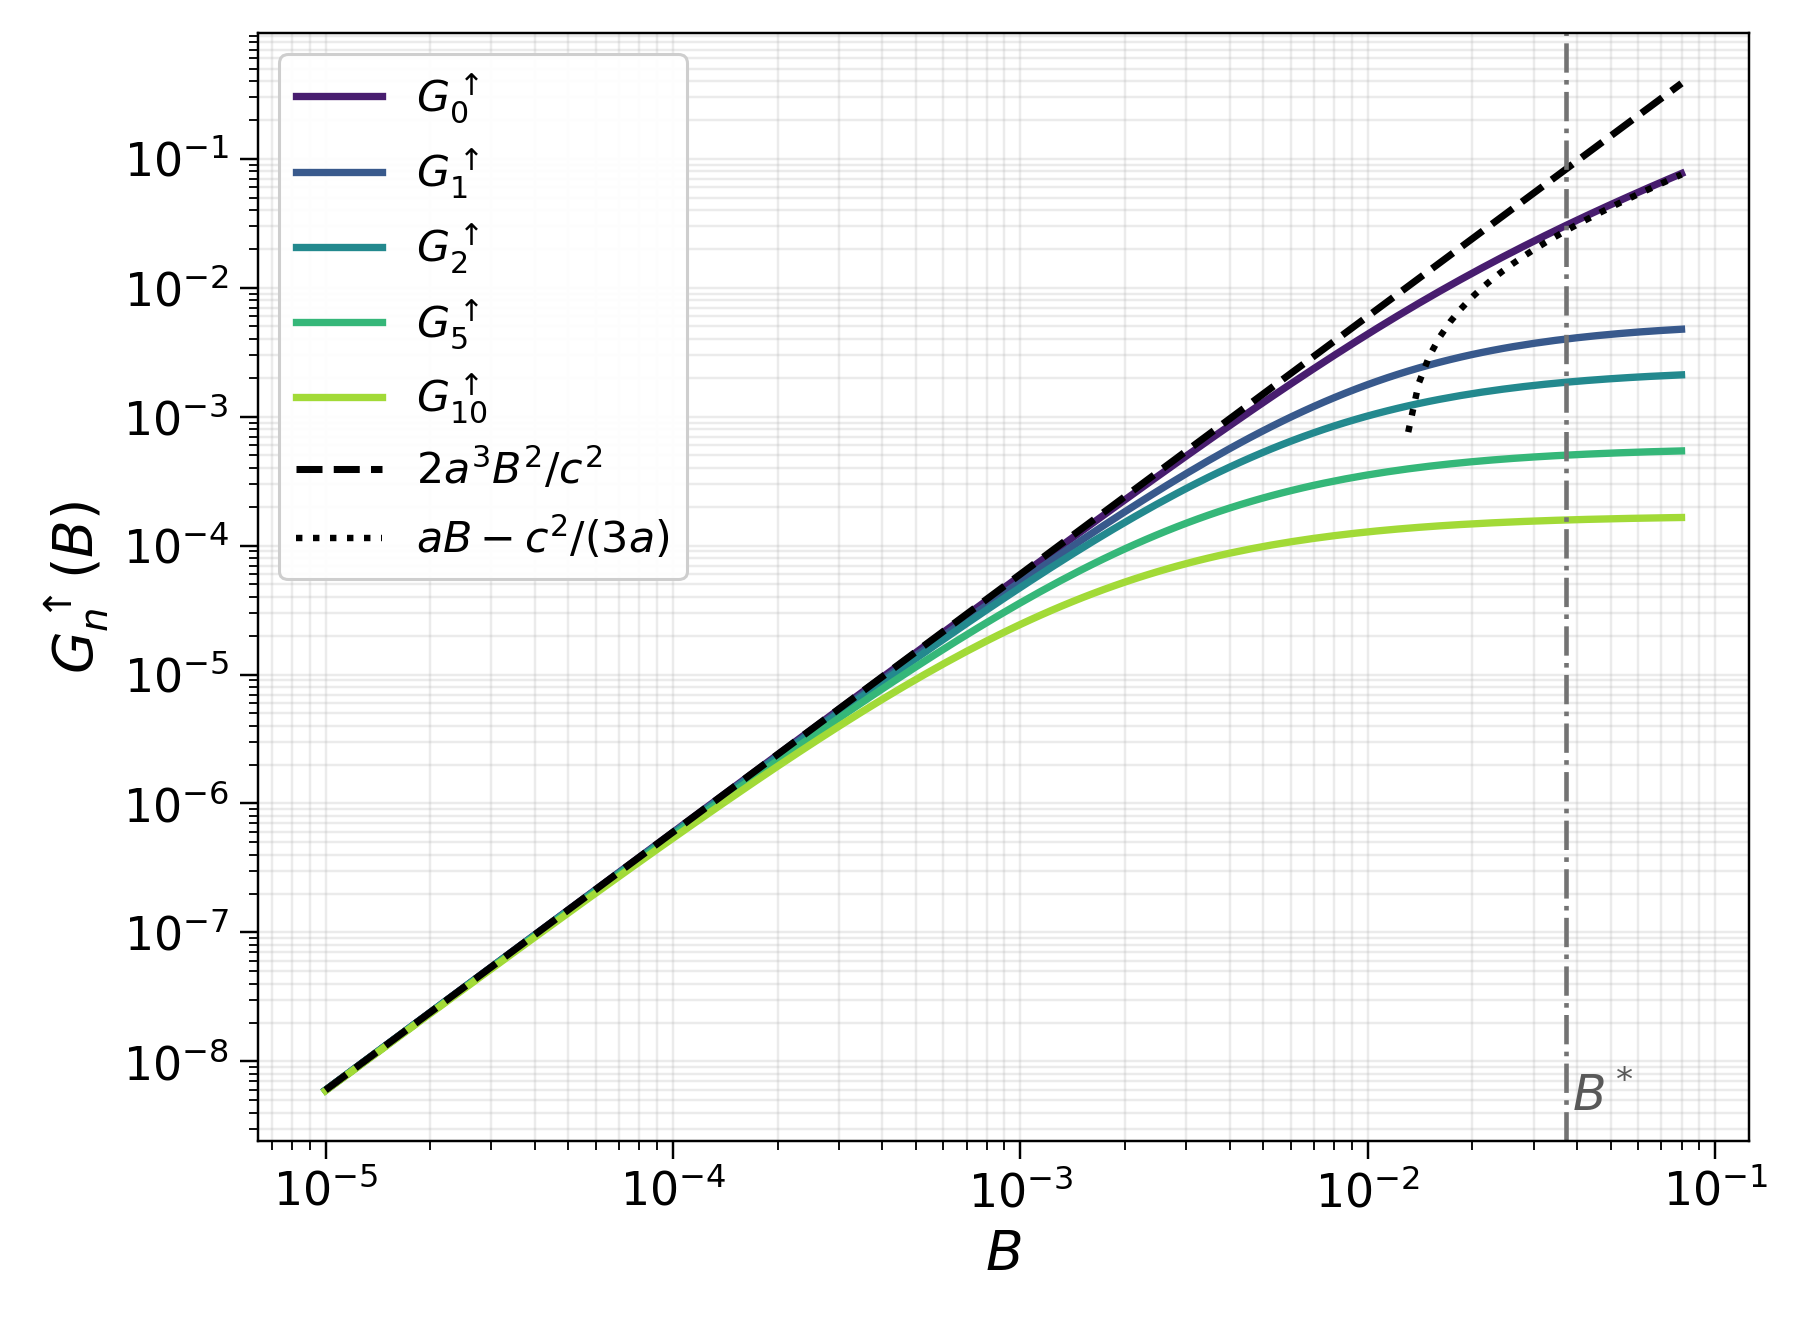
\includegraphics[width=\linewidth]{../figures/appendix_numerics_fresh/slide12_gap_b2_scaling.png}
    \caption{Exact fixed-index gap scaling from Eq.~\eqref{eq_SM:LL_gap_def} for the spin-up anomalous LL manifold. The dashed line shows the fixed-index low-field asymptote $2a^3B^2/c^2$, while the dotted line shows the large-field asymptote $aB-c^2/(3a)$ for the top gap. The vertical dash-dotted line marks $B^*=c^2/a^2$.}
    \label{fig:gap-scaling}
\end{figure}

% ================================================================
\section{Branch-Resolved LK Formulas}
\label{app:lk-branch}
\label{app:LL-spacing-formulas}

\subsection{Poisson-summation and contour evaluation}
\label{app:LK-derivation}

We outline the derivation of Eq.~\eqref{eq:omega-tilde} and Eq.~\eqref{eq:Xp-manuscript} of the main text from the exact LL spectrum.
For a LL branch labelled by spin sector $\alpha$ and band index $\eta=\pm$, with energies $E^\alpha_\eta(n,B)$ and degeneracy per unit area $D=B/(2\pi)$, the grand potential per unit area is
\begin{equation}
    \Omega(B,T,\mu)
    =
    -\kB T D \sum_{\alpha,\eta} \sum_{n=0}^{\Lmax}
    \ln\!\bigl[1+e^{-(E^\alpha_\eta(n,B)-\mu)/\kB T}\bigr].
    \label{eq:grand-potential-branch-app}
\end{equation}
Applying Poisson summation to this sum isolates the oscillatory part as
\begin{eqnarray}
    && \delta\Omega(B,T,\mu) = \sum_{\alpha,\eta} \delta\Omega_{\alpha,\eta}(B,T,\mu), \nonumber \\
    && \delta\Omega_{\alpha,\eta} (B,T,\mu) = -2 \kB T D\,\Re\sum_{p=1}^{\infty}
    \int_{-1/2}^{\Lmax+1/2} dn\,
    \ln \bigl[1+e^{-(E^\alpha_\eta(n,B)-\mu)/\kB T}\bigr]\,
    e^{2\pi\ii p n},
    \label{eq:omega-osc-raw}
\end{eqnarray}
with $D = B/(2\pi)$ and $\Re$ takes the real part.
Here the index $n$ is treated as a continuous variable, and the upper limit $\Lmax$ is set by the continuum cutoff.
Starting from this form, change variable to $\varepsilon=E^\alpha_\eta(n,B)$ with $dn=d\varepsilon/v_{\varepsilon}$, where 
\begin{eqnarray}
    v_{\varepsilon}=|\partial E^\alpha_\eta(n,B)/\partial n|_{n(\varepsilon)}
\end{eqnarray}
is the local LL spacing.
The temperature-dependent part of the integral is controlled by energies within a window of order $\kB T$ around the chemical potential.
When the local spacing varies slowly over this window, one may expand the inverse LL index $n_{\alpha,\eta}(\varepsilon,B)$ about the Fermi crossing $n^*_{\alpha,\eta}$ defined by 
\begin{eqnarray}
    E^\alpha_\eta(n^*_{\alpha,\eta},B)=\mu.    
\end{eqnarray}
Keeping the leading term gives
\begin{equation}
    n_{\alpha,\eta}(\varepsilon,B) \approx n^{*}_{\alpha,\eta} + \frac{\varepsilon-\mu}{v^{\alpha,\eta}_{\mu}},\qquad
    v^{\alpha,\eta}_\mu \equiv \bigl|\partial E^\alpha_\eta(n,B)/\partial n\bigr|_{n^*_{\alpha,\eta}},
\label{eq:vmu-def-app}
\end{equation}
where $v^{\alpha,\eta}_\mu$ is equivalent to the definition in Eq.~\eqref{eq:omega-tilde} of the main text.
Taking $v_{\varepsilon}\approx v^{\alpha,\eta}_{\mu}$ outside the integral gives
\begin{equation}
    \delta\Omega_{\alpha,\eta} \approx -\frac{2\kB T D}{v^{\alpha,\eta}_{\mu}}
    \Re\sum_{p=1}^{\infty} e^{2\pi\ii p n^{*}_{\alpha,\eta}}
    \int d\varepsilon
    \ln\!\bigl[1+e^{-(\varepsilon-\mu)/\kB T}\bigr]
    e^{2\pi\ii p (\varepsilon-\mu)/v^{\alpha,\eta}_{\mu}}.
    \label{eq:omega-after-approx}
\end{equation}

Due to the logarithm in Eq.~\eqref{eq:omega-after-approx}, we first need to consider the integral boundary. For $\xi=(\varepsilon-\mu)/(\kB T)\to-\infty$, $\ln(1+e^{-\xi})\sim-\xi$, so the boundary term from a direct integration by parts would not vanish.
Let $F(\xi)=\ln(1+e^{-\xi})$, $\tilde v = 2\pi p\kB T/v^{\alpha,\eta}_\mu$, and keep the finite dimensionless endpoints $\xi_\pm=(\varepsilon_\pm-\mu)/(\kB T)$ inherited from the LL cutoff.
For this finite interval, two integrations by parts give the exact identity
\begin{equation}
    \int_{\xi_-}^{\xi_+}d\xi\,F(\xi)e^{\ii\tilde v\xi}
    = {\cal B}_{\rm end}
    -\frac{1}{\tilde v^2}
    \int_{\xi_-}^{\xi_+}d\xi\,F''(\xi)e^{\ii\tilde v\xi},
    \qquad
    F''(\xi)=\frac{1}{4}\operatorname{sech}^2\!\left(\frac{\xi}{2}\right).
\end{equation}
Here ${\cal B}_{\rm end}$ contains only finite-endpoint terms evaluated at $\xi_\pm$.
These terms are cutoff/edge contributions, whereas the LK oscillation associated with the Fermi crossing is controlled by the nonanalytic change of occupation at $\varepsilon=\mu$ at zero temperature.
When the Fermi level is far from the endpoints on the scale of $\kB T$, the Fermi-surface contribution can therefore be isolated by extending the localized kernel $F''(\xi)$ to the full real line.
In the $T\to0$ limit, $F''(\xi)$ tends to $\delta(\xi)$, giving the undamped $T=0$ harmonic; at finite $T$ the broadened kernel gives the LK damping factor
\begin{align}
    R_T(\tilde v)
    &=
    \int_{-\infty}^{\infty} d\xi\,
    \left[-f'_0(\xi)\right]e^{\ii\tilde v\xi}
    =
    \int_{-\infty}^{\infty} \frac{d\xi}{4}
    \operatorname{sech}^2\!\!\left(\frac{\xi}{2}\right)e^{\ii\tilde v\xi},
\end{align}
where $f_0(\xi) = (1+e^\xi)^{-1}$. In this expression for $R_T(\tilde v)$, the imaginary part vanishes because the thermal kernel is even in $\xi$, whereas $\sin(\tilde v\xi)$ is odd.
Closing the contour in the upper half-plane picks up the Matsubara poles of $f'_0(\xi)$ at $\xi_k = \ii\pi(2k+1)$ ($k=0,1,2,\ldots$):
\begin{equation}
    R_T(\tilde v)
    = \frac{X^{\alpha,\eta}_p}{\sinh(X^{\alpha,\eta}_p)}.
\end{equation}
where 
\begin{eqnarray}
    X^{\alpha,\eta}_p \equiv \pi\tilde v = 2\pi^2 p \kB T/v^{\alpha,\eta}_\mu.
\end{eqnarray}
Collecting all prefactors -- the Jacobian $1/v^{\alpha,\eta}_\mu$ from the change of variable, two integration-by-parts factors of $v^{\alpha,\eta}_\mu/(2\pi p)$, and the explicit $D$ factor -- yields
\begin{equation}
    \delta\Omega_{\alpha,\eta}(B,T,\mu) = \frac{D}{2\pi^{2}}\sum_{p=1}^{\infty}\frac{v^{\alpha,\eta}_{\mu}}{p^{2}}
    \,\frac{X^{\alpha,\eta}_p}{\sinh X^{\alpha,\eta}_p}\,\cos\!\bigl[2\pi p\, n^{*}_{\alpha,\eta}(\mu, B)\bigr],
    \label{eq:branch-lk-omega-app}
\end{equation}
in agreement with Eq.~\eqref{eq:omega-tilde} of the main text.
(For complete bookkeeping, see e.g.\ Shoenberg, \emph{Magnetic Oscillations in Metals}, \S2.3, eqs.\ 2.151--2.157.)

\subsection{Local LL spacing for each branch}

\paragraph{$\ELLminus$ branch ($\mu>E_0$, wedge condition $0<\dmu<c\sqrt{B}$).}
Setting $\ELLminus(n^*,B) = \mu$ with $\dmu = \mu-E_0>0$ means
\begin{equation}
    2\dmu = U_{n^{*}} - \sqrt{U_{n^{*}}^{2} - 4c^{2}B}.
    \label{eq:cross-LL-app}
\end{equation}
Rearranging to isolate the square root and squaring:
$(U_{n^*}-2\dmu)^2 = U_{n^*}^2 - 4c^2B$, which gives $4\dmu^2 - 4\dmu U_{n^*} = -4c^2B$, hence
\begin{equation}
    U_{n^{*}} \equiv \frac{c^{2}}{a}+(2n^{*}+1)aB
    = \dmu + \frac{c^{2}B}{\dmu}.
    \label{eq:U-star-app}
\end{equation}
(The squaring step requires $U_{n^*}>2\dmu$, i.e.\ $c^2B>\dmu^2$, which is precisely the wedge condition.)
Solving Eq.~\eqref{eq:U-star-app} for $n^*$:
\begin{equation}
    n^{*} + \frac12
    = \frac{U_{n^*}-c^2/a}{2aB}
    = -\frac{E_0+c^2/a-\mu}{2aB} + \frac{c^{2}}{2a(\mu-E_0)}.
    \label{eq:nstar-LL-app}
\end{equation}
Here the combination $E_0+c^2/a$ enters only through the ideal-flat-band offset in the spin-up block.
The local spacing follows from $\partial E_{-}/\partial n\big|_{n^*}$. Differentiating $\ELLminus = E_0 + \tfrac12(U_n - \sqrt{U_n^2-4c^2B})$ with respect to $n$ (using $\partial U_n/\partial n = 2aB$) and evaluating at $n^*$ where $\sqrt{U_{n^*}^2-4c^2B} = U_{n^*}-2\dmu$:
\begin{equation}
    \frac{\partial \ELLminus}{\partial n}\bigg|_{n^{*}}
    = aB\!\left(1 - \frac{U_{n^*}}{U_{n^*}-2\dmu}\right)
    = \frac{-2aB\,\dmu}{U_{n^*}-2\dmu}
    = \frac{-2aB\,\dmu^2}{c^2B-\dmu^2},
\end{equation}
where we used $U_{n^*}-2\dmu = (c^2B-\dmu^2)/\dmu$ from Eq.~\eqref{eq:U-star-app}.
Since $\dmu < c\sqrt{B}$, the denominator $c^2B-\dmu^2>0$ and the slope is negative (levels decrease in $n$).
Taking the absolute value of this local slope gives the positive LL spacing:
\begin{equation}
    v_{\mu}^{\uparrow,-} \equiv \Bigl|\frac{\partial \ELLminus}{\partial n}\Bigr|_{n^{*}}
    = \frac{2aB(\mu-E_0)^{2}}{c^{2}B - (\mu-E_0)^{2}}.
    \label{eq:dEdn-LLminus-app}
\end{equation}

\paragraph{$\ELLTRminus$ branch ($\mu<E_0$, valid for $-c\sqrt{B}<\dmu<0$).}
Setting $\ELLTRminus(n^*,B) = \mu$ with $\dmu = \mu-E_0<0$:
\begin{equation}
    2\dmu = V_{n^{*}} - \sqrt{V_{n^{*}}^{2} + 4c^{2}B}.
    \label{eq:cross-LLTR-app}
\end{equation}
Isolating the square root and squaring: $(V_{n^*}-2\dmu)^2 = V_{n^*}^2+4c^2B$, giving
$4\dmu^2 - 4\dmu V_{n^*} = 4c^2B$, hence (with $\dmu<0$)
\begin{equation}
    V_{n^{*}} \equiv \frac{c^{2}}{a}+(2n^{*}-1)aB
    = \dmu - \frac{c^{2}B}{\dmu}.
    \label{eq:V-star-app}
\end{equation}
Solving for $n^*$:
\begin{equation}
    n^{*} - \frac12
    = \frac{V_{n^*}-c^2/a}{2aB}
    = \frac{c^{2}}{2a(E_0-\mu)} - \frac{E_0+c^2/a-\mu}{2aB}.
    \label{eq:nstar-LLTR-app}
\end{equation}
The local spacing can be obtained directly from the slope of the spin-down anomalous branch.
Differentiating $\ELLTRminus = E_0+\tfrac12(V_n-\sqrt{V_n^2+4c^2B})$ with respect to $n$ and using $\partial V_n/\partial n=2aB$ gives
\begin{equation}
    \frac{\partial \ELLTRminus}{\partial n}\bigg|_{n^*}
    =
    aB\!\left(1-\frac{V_{n^*}}{\sqrt{V_{n^*}^2+4c^2B}}\right).
\end{equation}
At the Fermi crossing, Eq.~\eqref{eq:cross-LLTR-app} gives
$\sqrt{V_{n^*}^2+4c^2B}=V_{n^*}-2\dmu$.
Using Eq.~\eqref{eq:V-star-app},
\begin{equation}
    V_{n^*}-2\dmu
    =
    -\dmu-\frac{c^2B}{\dmu}
    =
    -\frac{\dmu^2+c^2B}{\dmu},
\end{equation}
which is positive because $\dmu<0$.
Therefore
\begin{equation}
    \frac{\partial \ELLTRminus}{\partial n}\bigg|_{n^*}
    =
    aB\left[1+
    \frac{\dmu^2-c^2B}{\dmu^2+c^2B}\right]
    =
    \frac{2aB\dmu^2}{\dmu^2+c^2B}.
\end{equation}
The slope is positive for this branch, so the positive local spacing is
\begin{equation}
    v_{\mu}^{\downarrow,-} \equiv \Bigl|\frac{\partial \ELLTRminus}{\partial n}\Bigr|_{n^{*}}
    = \frac{2aB(\mu-E_0)^{2}}{(\mu-E_0)^{2} + c^{2}B}.
    \label{eq:dEdn-LLTR-app}
\end{equation}

\paragraph{Semiclassical (bulk) limit and connection to quantum geometry.}
In the bulk of the anomalous manifold ($|\dmu|\ll c\sqrt{B}$, large $n^*$), Eq.~\eqref{eq:dEdn-LLminus-app} first reduces to
\begin{equation}
    v_{\mu}^{\uparrow,-}
    =\frac{2aB\dmu^2}{c^2B-\dmu^2}
    \approx \frac{2a\dmu^2}{c^2}.
\end{equation}
To relate $\dmu$ to the zero-field band geometry, use the large-$n^*$ semiclassical identification $k_{n^*}^2\approx 2n^*B$.
In the same regime the anomalous LL energy follows from expanding the lower branch as
\begin{equation}
    \dmu = \ELLminus(n^*,B)-E_0
    \approx \frac{c^2B}{U_{n^*}}
    \approx \frac{c^2B}{\Delta(k_{n^*})},
    \qquad
    \Delta(k)=ak^2+\frac{c^2}{a},
\end{equation}
where we have used Eq.\eqref{eq_SM:ELLminus-approx}. 
Substituting this estimate for $\dmu$ into the bulk expression for $v_\mu$ gives
\begin{equation}
    v_{\mu}^{\uparrow,-} \approx \frac{2a\dmu^2}{c^2}
    \approx \frac{2ac^2B^2}{\Delta(k_{n^*})^2}
    = aB^2\,\tr\metric(k_{n^*}),
    \label{eq:v-geom-app}
\end{equation}
where the last equality uses $\tr\metric = 2c^2/\Delta^2$ from Eq.~\eqref{eq:g-and-Omega}.
The same relation holds for the $\ELLTRminus$ branch. Thus the local LL spacing directly encodes the quantum metric of the flat band, establishing $v^{\alpha,-}_\mu \sim aB^2 \tr\metric$ as the fundamental connection between anomalous-LL thermal damping and quantum geometry.

\paragraph{Upper branches ($\ELLplus$, $\ELLTRplus$).}
For the upper branches, the same differentiation of the exact LL energies gives
\begin{equation}
    v_{\mu}^{\uparrow,+}
    =
    \frac{2aB(\mu-E_0)^{2}}{(\mu-E_0)^{2}-c^{2}B},
    \qquad
    v_{\mu}^{\downarrow,+}
    =
    \frac{2aB(\mu-E_0)^{2}}{(\mu-E_0)^{2}+c^{2}B}.
    \label{eq:dEdn-upper-app}
\end{equation}
In the dispersive regime $|\mu-E_0|\gg c\sqrt{B}$, both upper-branch spacings reduce to $v^{\alpha,+}_{\mu}\approx 2aB$, recovering the standard parabolic-band LK factor $X^{\alpha,+}_p = \pi^{2} p \kB T/(aB)$ with effective mass $m^*_{\mathrm{eff},\alpha +} = 1/(2a)$.

\subsection{Effective mass formulas}

Using $\meff = B/v_{\mu}$ and the above expressions for $v_{\mu}$ gives:
\begin{align}
    m^{*}_{\mathrm{eff},\uparrow-}   & = \frac{c^{2}B - (\mu-E_0)^{2}}{2a(\mu-E_0)^{2}}, \label{eq:meff-LLminus-app}  \\
    m^{*}_{\mathrm{eff},\downarrow-} & = \frac{1}{2a} + \frac{c^{2}B}{2a(\mu-E_0)^{2}}. \label{eq:meff-LLTRminus-app}
\end{align}
In the anomalous bulk regime, $\dmu^2\ll c^2B$, the two lower-branch masses have the same leading behavior,
\begin{equation}
    m^*_{\mathrm{eff},\uparrow-}
    \simeq
    m^*_{\mathrm{eff},\downarrow-}
    \simeq
    \frac{c^2B}{2a(\mu-E_0)^2},
    \label{eq:meff-anomalous-bulk-app}
\end{equation}
up to the subleading additive constants $\mp 1/(2a)$.
This strong field dependence at fixed $\mu$ contrasts with the constant parabolic value $m^*_{\mathrm{eff},\alpha +}=1/(2a)$ of the dispersive upper branches.
At fixed carrier density, however, the field dependence must be evaluated along the self-consistent trajectory $\mu_\rho(B)$.
For a single active lower-branch sequence, the LL degeneracy is $D=B/(2\pi)$, so fixed active density $\rho_{\mathcal S}$ (defined in Sec.~D as the density counted by the active sector) selects
\begin{equation}
    n^*(B)\simeq \frac{|\rho_{\mathcal S}|}{D}
    =
    \frac{2\pi|\rho_{\mathcal S}|}{B}.
    \label{eq:nstar-fixed-density-app}
\end{equation}
The semiclassical momentum tied to this crossing is therefore
\begin{equation}
    k_{n^*}^2\simeq 2n^*B\simeq 4\pi|\rho_{\mathcal S}|,
    \label{eq:kn-fixed-density-app}
\end{equation}
which is approximately independent of $B$ at fixed density.
Using the weak-field anomalous-branch dispersion,
\begin{equation}
    \mu_\rho(B)-E_0
    \simeq
    s_\alpha\frac{c^2B}{c^2/a+a k_{n^*}^2}
    \simeq
    s_\alpha\frac{c^2}{c^2/a+4\pi a|\rho_{\mathcal S}|}\,B,
    \qquad
    s_\uparrow=+1,\quad s_\downarrow=-1,
    \label{eq:mu-fixed-density-linear-app}
\end{equation}
so the chemical-potential offset from the flat-band energy is linear in $B$ along the fixed-density trajectory.
Substituting Eq.~\eqref{eq:mu-fixed-density-linear-app} into Eq.~\eqref{eq:meff-anomalous-bulk-app} gives
\begin{equation}
    m^*_{\mathrm{eff},\alpha-}\bigl(B,\mu_\rho(B)\bigr)
    \simeq
    \frac{\left(c^2/a+4\pi a|\rho_{\mathcal S}|\right)^2}{2ac^2}\,\frac{1}{B}
    =
    \frac{1}{aB\,\tr\metric_\alpha(k_{n^*})},
    \label{eq:meff-fixed-density-inverseB-app}
\end{equation}
which is the roughly $1/B$ trend shown by the dashed theory curves in Fig.~\ref{fig:main4} of the main text.

% ================================================================
\section{Numerical Results for Fixed-Density Thermodynamics}
\label{app:thermodynamics}

\subsection{Density convention and Fermi level}

We first fix the density convention used in all numerical plots.
The signed carrier density \(\rho\) is measured relative to the midpoint of the two zero modes,
\begin{equation}
    E_{\mathrm{ref}}(B)=\frac{\ELLzero(B)+\ELLTRzero(B)}{2}.
    \label{eq:Eref-app}
\end{equation}
Thus \(\rho>0\) denotes electron doping above \(E_{\mathrm{ref}}\), while \(\rho<0\) denotes hole doping below \(E_{\mathrm{ref}}\).
The corresponding discrete LL spectral density per unit area is
\begin{equation}
    \nu_{\mathrm{LL}}(E,B) =
    \frac{B}{2\pi}
    \left[
    \sum_{\alpha=\uparrow,\downarrow}
    \delta\!\left(E-E^\alpha_0(B)\right)
    +
    \sum_{\alpha=\uparrow,\downarrow}
    \sum_{\eta=\pm}
    \sum_{n=1}^{\Lmax}
    \delta\!\left(E-E^\alpha_\eta(n,B)\right)
    \right],
    \label{eq:LL-spectral-density-app}
\end{equation}
where \(E^\alpha_0(B)\) denotes the zero mode in spin sector \(\alpha\), and \(E^\alpha_\eta(n,B)\) denotes the branch-resolved LL energy introduced in Appendix~\ref{app:LL-spectrum}.
At finite temperature, the signed density associated with a chemical potential \(\mu\) is obtained by integrating the LL spectral density with the Fermi occupation,
\begin{equation}
    \rho(\mu,B,T)
    =
    \int dE\,
    \nu_{\mathrm{LL}}(E,B)
    \left[
    f_T(E-\mu)-\Theta\!\left(E_{\mathrm{ref}}(B)-E\right)
    \right],
    \qquad
    f_T(x)=\frac{1}{e^{x/\kB T}+1}.
    \label{eq:finiteT-density-app}
\end{equation}
The second term subtracts the reference filling with all LLs below \(E_{\mathrm{ref}}\) occupied and all LLs above \(E_{\mathrm{ref}}\) empty.
For a prescribed carrier density, the chemical potential \(\mu_\rho(B,T)\) is determined by solving \(\rho=\rho(\mu_\rho,B,T)\).
In the \(T\to0\) limit, Eq.~\eqref{eq:finiteT-density-app} reduces to the usual signed LL-counting convention relative to \(E_{\mathrm{ref}}\).

Since we need to choose a momentum cutoff $\Lambda$ for the topological flat bands, which also introduces a cutoff in the anomalous LL spectrum, it is more stable to work with the active carrier sector rather than with the full signed integral each time.
This gives three cases:
\begin{align}
    \rho>0:\quad
    &\rho_{\mathcal S}=\rho,
    &&\mathcal{S}=\{\text{electron LLs above }E_{\mathrm{ref}}\},
    \notag\\
    -\rho_{\mathrm{cap}}/2<\rho<0:\quad
    &\rho_{\mathcal S}=|\rho|,
    &&\mathcal{S}=\{\text{hole levels counted downward from }E_{\mathrm{ref}}\},
    \notag\\
    \rho<-\rho_{\mathrm{cap}}/2:\quad
    &\rho_{\mathcal S}=\rho_{\mathrm{low},e}
    =\rho_{\mathrm{cap}}-|\rho|,
    &&\mathcal{S}=\{\text{remaining electrons in the lower manifold}\}.
    \label{eq:density-regimes-app}
\end{align}
The shallow-hole description is used when the missing carriers are still between \(E_0\) and \(E_{\mathrm{ref}}\), so the chemical potential is within the upper manifold of anomalous LLs. The maximal carrier density of the two anomalous sectors together is 
\begin{equation}
    \rho_{\mathrm{cap}}=\frac{\Lambda^2}{2\pi}.
    \label{eq:rho-cap-app}
\end{equation}
Thus the shallow/deep boundary in Eq.~\eqref{eq:density-regimes-app} occurs at \(\rho_{\mathrm{cap}}/2=\Lambda^2/(4\pi)\).
For \(\Lambda=1.0\,\mathrm{nm}^{-1}\), one flat band has capacity \(0.0796\,\mathrm{nm}^{-2}\), while the combined two-sector capacity is \(\rho_{\mathrm{cap}}=0.159\,\mathrm{nm}^{-2}\); therefore \(\rho=-0.140\) and \(-0.150\,\mathrm{nm}^{-2}\) are deep-hole examples used below for numerical calculations in this combined convention.
This rewriting is only a carrier-counting convention: the oscillations are then controlled by the small number \(\rho_{\mathrm{low},e}\) of lower-manifold electrons left unremoved.
Consequently, the black reference lines in the FFT plots use \(F=2\pi|\rho|\) for the electron and shallow-hole sectors, whereas the deep-hole reference uses \(F=2\pi\rho_{\mathrm{low},e}\).
As discussed below, the \(\rho=+0.020\,\mathrm{nm}^{-2}\) magnetization
spectrum also contains a dominant low-frequency peak near \(F=\pi\rho\).
This feature correlates with the near-Fermi LL splitting structure and does
not alter the fixed-density counting convention.

For each case in Eq.~\eqref{eq:density-regimes-app}, we introduce an active-sector energy variable \(\varepsilon^{\mathcal S}_\ell(B)\).
Let \(E_\ell(B)\) denote the LL energies \(E^\alpha_0(B)\) and \(E^\alpha_\eta(n,B)\) in the original electron spectrum.
Then
\begin{equation}
    \varepsilon^{\mathcal S}_\ell(B)=
    \begin{cases}
    E_\ell(B), & \mathcal S=\{\text{electron LLs above }E_{\mathrm{ref}}\},\\
    E_{\mathrm{ref}}(B)-E_\ell(B), & \mathcal S=\{\text{hole levels counted downward from }E_{\mathrm{ref}}\},\\
    E_\ell(B), & \mathcal S=\{\text{remaining electrons in the lower manifold}\}.
    \end{cases}
    \label{eq:sector-energy-app}
\end{equation}
The sector density \(\rho_{\mathcal S}\) is therefore the active carrier density for the chosen sector.
Only after this sector energy variable is fixed do we define the sector chemical potential \(\mu_{\mathcal S}\).
It is the quantity conjugate to \(\rho_{\mathcal S}\), measured in the same energy variable as \(\varepsilon^{\mathcal S}_\ell\), and is defined implicitly by
\begin{equation}
    \rho_{\mathcal S}
    =
    D\sum_{\ell\in\mathcal S}
    f_T\!\left(\varepsilon^{\mathcal S}_\ell(B)-\mu_{\mathcal S}\right),
    \qquad
    D=\frac{B}{2\pi},
    \label{eq:sector-density-app}
\end{equation}
which is the sector version of Eq.~\eqref{eq:finiteT-density-app}.
For the electron and deep-hole sectors, \(\mu_{\mathcal S}\) is the physical electron chemical potential restricted to the retained sector.
For the shallow-hole sector, \(\mu_{\mathcal S}\) is instead the hole chemical potential in the transformed variable \(E_{\mathrm{ref}}-E_\ell\), not the original electron chemical potential \(\mu\).

\subsection{Fixed-density magnetization}

For each active carrier sector $\mathcal{S}$, the sector grand potential is
\begin{equation}
    \Omega_{\mathcal{S}}(B,T,\mu_{\mathcal{S}})
    = -\kB T\,D\sum_{\ell\in\mathcal{S}}
    \ln\!\left[1+\exp\!(-\frac{\varepsilon^{\mathcal{S}}_\ell(B)-\mu_{\mathcal{S}}}{\kB T})\right],
    \label{eq:omega-sector}
\end{equation}
Here $\mathcal{S}$, \(\varepsilon^{\mathcal{S}}_\ell(B)\), \(\rho_{\mathcal S}\), \(\mu_{\mathcal{S}}(B,T,\rho_{\mathcal{S}})\), and \(D\) are the sector quantities defined above.
The magnetization (per unit area) at fixed sector density is obtained from the Helmholtz free energy $f_{\mathcal{S}} = \Omega_{\mathcal{S}} + \mu_{\mathcal{S}}\rho_{\mathcal{S}}$:
\begin{equation}
    M_{\mathcal{S}}(B,T,\rho_{\mathcal{S}}) = -\frac{\partial f_{\mathcal{S}}}{\partial B}\bigg|_{T,\rho_{\mathcal{S}}}.
    \label{eq:M-sector}
\end{equation}
To see how the fixed-density derivative is evaluated, write the chemical potential on the fixed-density trajectory as \(\mu_{\mathcal S}(B)\), suppressing \(T\) and \(\rho_{\mathcal S}\) in the notation.
Then
\begin{align}
    \frac{d f_{\mathcal S}}{dB}\bigg|_{T,\rho_{\mathcal S}}
    &=
    \left(\frac{\partial \Omega_{\mathcal S}}{\partial B}\right)_{T,\mu_{\mathcal S}}
    +
    \left(\frac{\partial \Omega_{\mathcal S}}{\partial \mu_{\mathcal S}}\right)_{T,B}
    \frac{d\mu_{\mathcal S}}{dB}
    +
    \rho_{\mathcal S}\frac{d\mu_{\mathcal S}}{dB}
    \notag\\
    &=
    \left(\frac{\partial \Omega_{\mathcal S}}{\partial B}\right)_{T,\mu_{\mathcal S}},
    \label{eq:fixed-density-cancel-app}
\end{align}
where the last equality uses the thermodynamic identity \(\rho_{\mathcal S}=-(\partial\Omega_{\mathcal S}/\partial\mu_{\mathcal S})_{T,B}\).
Thus \(M_{\mathcal S}\) can equivalently be computed as \(-(\partial\Omega_{\mathcal S}/\partial B)_{T,\mu_{\mathcal S}}\) evaluated at \(\mu_{\mathcal S}=\mu_{\mathcal S}(B,T,\rho_{\mathcal S})\).
In the numerical evaluation, the \(B\)-derivative in Eq.~\eqref{eq:fixed-density-cancel-app} can be obtained analytically from the explicit LL energies \(E^\alpha_0(B)\) and \(E^\alpha_\eta(n,B)\) given in Appendix~\ref{app:LL-spectrum}.

The oscillatory part $\widetilde{M}$ is obtained numerically by subtracting a smooth background in $1/B$.
For the anomalous densities, we adopt the $M_{\text{no0LL}}$ convention: the zero-mode contributions are excluded from the oscillatory signal to avoid contamination by the field-independent $\ELLTRzero$ and the trivial $B$-linear $\ELLzero$ shift, which has no contribution to oscillation behaviors.
We also evaluate the exact discrete sector grand potential in Eq.~\eqref{eq:omega-sector} along the fixed-density trajectory and subtract the same type of smooth background, denoting the resulting oscillatory component by $\delta\Omega_{\rho}$.
For deep-hole densities, the active density is the remaining lower-manifold electron density defined in Eq.~\eqref{eq:density-regimes-app}.
This construction is shown directly in Fig.~\ref{fig:thermo-wide-osc}, which plots the resulting thermodynamic oscillations over a wide \(1/B\) range for the six densities used in the appendix.
The left column shows the background-subtracted grand potential \(\delta\Omega_\rho\) obtained from the exact LL sum, while the right column shows the background-subtracted, zero-mode-excluded magnetization \(\widetilde M_{\mathrm{no0LL}}\).
Thus Fig.~\ref{fig:thermo-wide-osc} serves as the starting point for the subsequent FFT, window, and thermal-damping analyses, and it also makes the temperature dependence visible before any Fourier or local-window processing is applied. 
At the lowest temperatures, the electron densities in the dispersive regime, Figs.~\ref{fig:thermo-wide-osc}(a)--\ref{fig:thermo-wide-osc}(d), show many well-resolved oscillation periods across the plotted \(1/B\) range, whereas the hole densities in the anomalous regime, Figs.~\ref{fig:thermo-wide-osc}(e)--\ref{fig:thermo-wide-osc}(l), lose amplitude rapidly toward smaller \(B\) (larger \(1/B\)), leaving only a few visible periods before the oscillatory signal becomes strongly suppressed.


\begin{figure}[htbp]
    \centering
    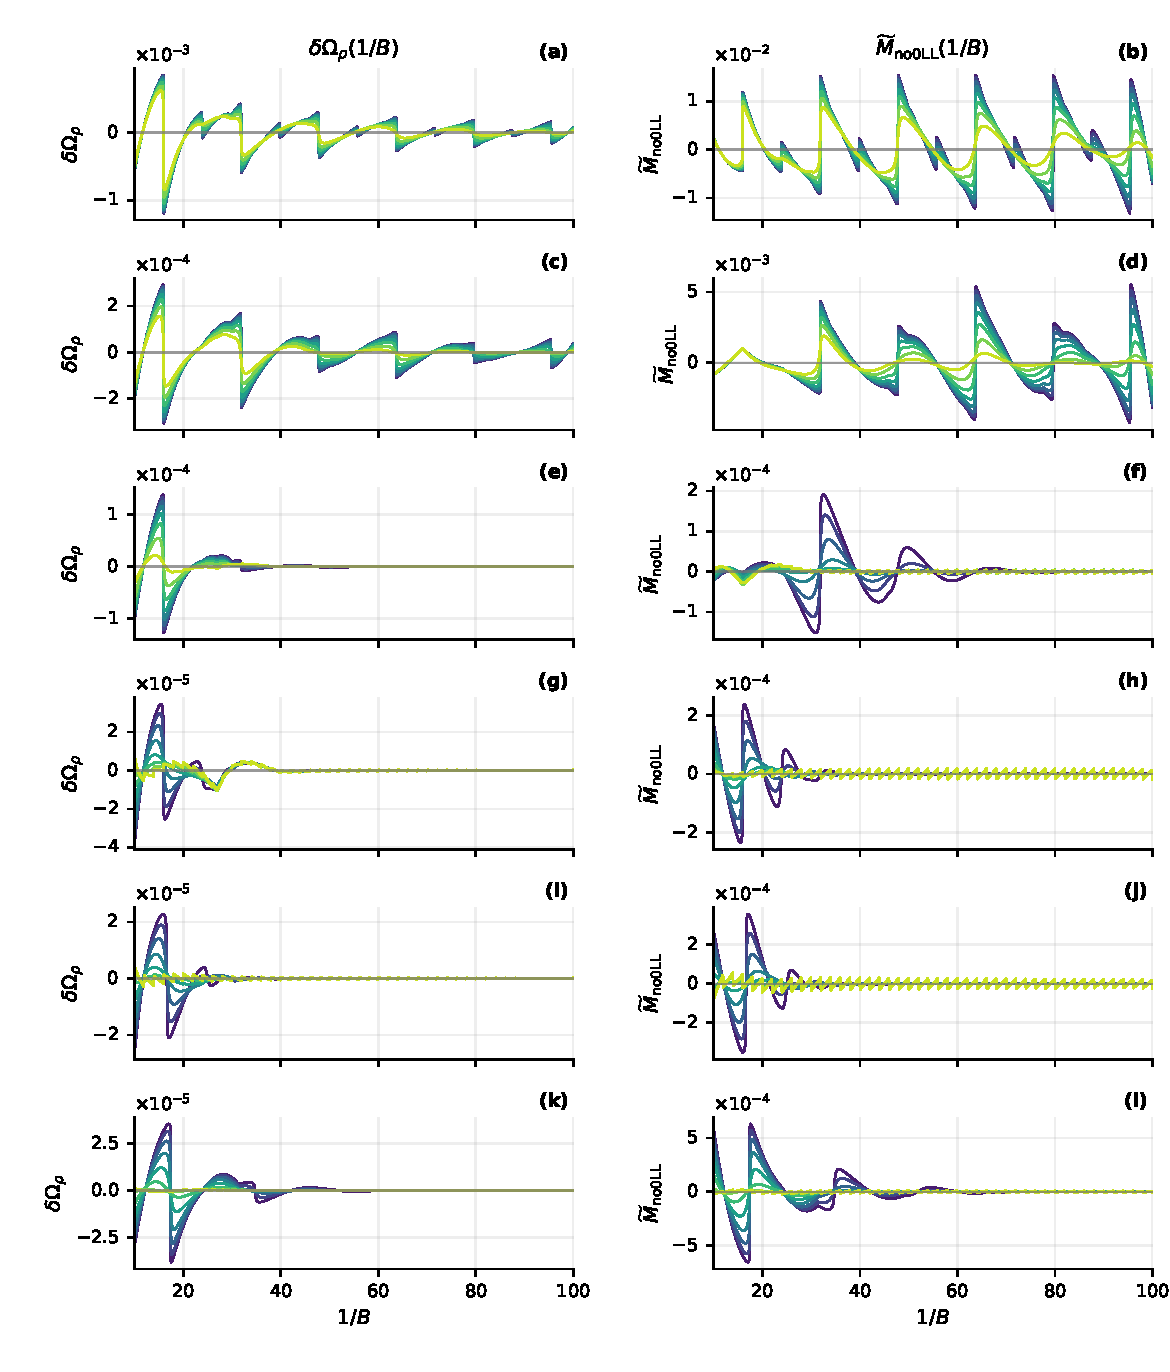
\includegraphics[width=\linewidth]{../figures/appendix_numerics_fresh/appD1_lambda1_deltaOmega_M_wide.pdf}
    \caption{Wide-range thermodynamic oscillations at $\Lambda=1.0\,\mathrm{nm}^{-1}$ for $1/B\in[10,100]$. In each panel, the curves correspond to $k_B T=(2.00,\,3.07,\,4.71,\,7.22,\,11.1,\,17.0,\,26.1,\,40.0)\times10^{-4}\,\mathrm{eV}$, ordered from purple at the lowest temperature to yellow at the highest temperature. The left column shows the background-subtracted sector grand potential $\delta\Omega_{\rho}(1/B)$ computed from the exact discrete LL sum in Eq.~\eqref{eq:omega-sector}; the right column shows the background-subtracted, zero-mode-excluded oscillatory magnetization $\widetilde M_{\mathrm{no0LL}}(1/B)$ computed along the same fixed-density trajectory. The density assignments are $(a,b)$ $\rho=+0.020$, $(c,d)$ $\rho=+0.010$, $(e,f)$ $\rho=-0.010$, $(g,h)$ $\rho=-0.020$, $(i,j)$ $\rho=-0.140$, and $(k,l)$ $\rho=-0.150$, all in units of $\mathrm{nm}^{-2}$.}
    \label{fig:thermo-wide-osc}
\end{figure}

\subsection{FFT frequency diagnostics}

Figure~\ref{fig:magnetization-fft} is the frequency-space diagnostic of the wide-range oscillations in Fig.~\ref{fig:thermo-wide-osc}.
For each density, we Fourier transform the lowest-temperature traces, \(k_B T=2.0\times10^{-4}\,\mathrm{eV}\), using the same \(1/B\) interval as in Fig.~\ref{fig:thermo-wide-osc}.
The left column analyzes the background-subtracted grand potential \(\delta\Omega_\rho\), while the right column analyzes the background-subtracted, zero-mode-excluded magnetization \(\widetilde M_{\mathrm{no0LL}}\).
The vertical dashed lines in Fig.~\ref{fig:magnetization-fft} are LL-counting reference frequencies used to interpret where the numerical FFT weight should appear, as discussed below. 

For one set of LL ladder, the degeneracy per unit area is \(D=B/(2\pi)\).
If \(n_f\) levels are filled, the active carrier density is \(\rho_{\mathcal S}=D n_f\), so \(n_f=(2\pi\rho_{\mathcal S})/B\).
One oscillation occurs when \(n_f\) changes by one as a function of \(1/B\), giving the fundamental frequency
\begin{equation}
    F_{\rho_{\mathcal S}} = 2\pi\rho_{\mathcal S}.
    \label{eq:onsager-freq-app}
\end{equation}
Here \(\rho_{\mathcal S}\) is the density counted by the active LL sequence.
For the electron and shallow-hole rows, \(\rho_{\mathcal S}=|\rho|\).
For the deep-hole rows, the useful active variable is the remaining lower-manifold electron density \(\rho_{\mathcal S}=\rho_{\mathrm{low},e}\) defined in Eq.~\eqref{eq:density-regimes-app}, because the oscillations count the residual unfilled part of the lower anomalous manifold rather than the full hole density.
The black dashed lines in Fig.~\ref{fig:magnetization-fft} mark \(F=2\pi\rho_{\mathcal S}\) for both electron and hole sectors.
With this convention, the FFT spectra test whether the exact fixed-density LL calculation oscillates with the period expected from the active carrier density.
The electron-side spectra are shown first in Figs.~\ref{fig:magnetization-fft}(a)--\ref{fig:magnetization-fft}(d).
For \(\rho=+0.010\,\mathrm{nm}^{-2}\), panels (c) and (d) have their dominant peak consistent with the black line from Eq.~\eqref{eq:onsager-freq-app}, so the oscillations are well described by a spin-resolved LL ladder with \(\rho_{\mathcal S}=\rho\).
For \(\rho=+0.020\,\mathrm{nm}^{-2}\), panels (a) and (b) instead show a stronger low-frequency peak described by the green dashed line \(F=\pi\rho\), rather than by the black dashed line at \(F=2\pi\rho\).
This additional peak is consistent with an effectively spin-degenerate
density-frequency relation. If two spin ladders are sufficiently close over
the relevant field interval, the fixed total carrier density is shared between
them.
If \(g_s\) spin ladders contribute with the same frequency, each ladder carries \(\rho/g_s\), and Eq.~\eqref{eq:onsager-freq-app} gives
\begin{eqnarray}
    F = 2\pi\frac{\rho}{g_s}.
\end{eqnarray}
Thus an effectively spin-degenerate electron sequence with \(g_s=2\) gives
\(F=\pi\rho\), motivating the green guide in panels (a) and (b). The FFT alone
does not establish a unique degeneracy assignment. It instead indicates that
the \(\rho=+0.010\,\mathrm{nm}^{-2}\) trace is closer to the spin-resolved
counting scale, whereas the \(\rho=+0.020\,\mathrm{nm}^{-2}\) trace contains a
strong spin-degenerate-like component. We therefore examine the fixed-density
chemical potential and the nearest-Fermi LL spacing in
Fig.~\ref{fig:electron-mu-splitting-comparison} as a direct LL-level diagnostic
of the different electron-side spectra in
Figs.~\ref{fig:magnetization-fft}(a)--\ref{fig:magnetization-fft}(d).
Panel (a) shows that the fixed-density chemical potential is determined from the same full spin-sector LL spectrum for both \(\rho=+0.010\) and \(+0.020\,\mathrm{nm}^{-2}\).
Panel (b) then compares the nearest-Fermi-energy LL spacing \(\Delta E_{\mathrm{near}}\), defined by the two LLs immediately below and above \(\mu_{\mathcal S}\).
For \(\rho=+0.010\,\mathrm{nm}^{-2}\), the near-Fermi spacing is comparatively
regular, consistent with the dominant FFT weight near the spin-resolved
counting scale \(F=2\pi\rho\). For
\(\rho=+0.020\,\mathrm{nm}^{-2}\), \(\Delta E_{\mathrm{near}}\) has a much
stronger oscillatory modulation over the same \(1/B\) range, alternating
between small spin splittings and larger inter-LL spacings. The corresponding
chemical-potential modulation is visible in panel (a) of
Fig.~\ref{fig:electron-mu-splitting-comparison}. Together, these observations
support---without uniquely proving---the spin-degenerate-like interpretation
of the low-frequency FFT component.



On the hole side, the anomalous LLs from the two spin sectors are split into branches on opposite sides of \(E_0\), so they do not form the same kind of nearly spin-degenerate sequence that appears for the electron-side dispersive LLs.
The FFT spectra in Figs.~\ref{fig:magnetization-fft}(e)--\ref{fig:magnetization-fft}(l) therefore generally show one main counting peak.
Compared with the electron-side spectra, however, the hole-side peaks are much broader.
For \(\rho=-0.020\) and \(-0.140\,\mathrm{nm}^{-2}\), the \(\delta\Omega_\rho\) spectra in panels (g) and (i) are so broad that the peak position is difficult to assign reliably.
This is consistent with the direct \(1/B\)-domain traces in Fig.~\ref{fig:thermo-wide-osc}(g,i), where the \(\delta\Omega_\rho\) oscillations decay rapidly as \(1/B\) increases.
The corresponding magnetization spectra in Figs.~\ref{fig:magnetization-fft}(h) and \ref{fig:magnetization-fft}(j) still show visible peaks, but these peaks remain broader.
For \(\rho=-0.010\) and \(-0.150\,\mathrm{nm}^{-2}\), the main FFT peaks can be resolved in both \(\delta\Omega_\rho\) and \(\widetilde M_{\mathrm{no0LL}}\), and their positions are consistent with the active-density counting frequency \(F=2\pi\rho_{\mathcal S}\) in Eq.~\eqref{eq:onsager-freq-app}, shown by the black dashed lines.


\begin{figure}[htbp]
    \centering
    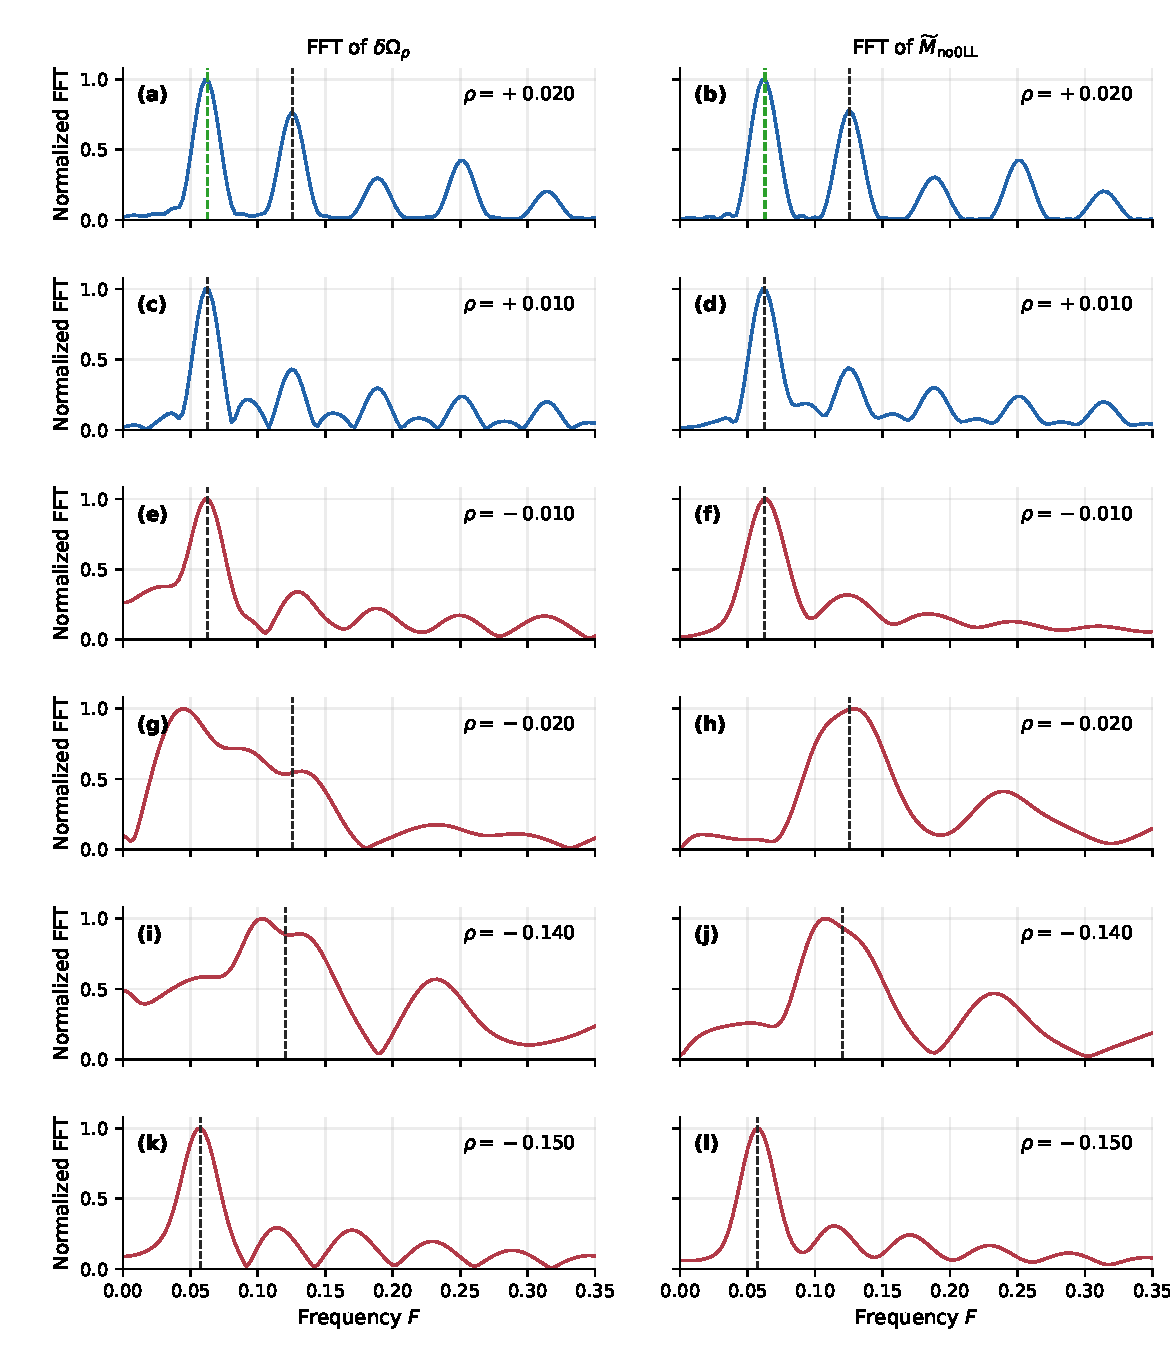
\includegraphics[width=\linewidth]{../figures/appendix_numerics_fresh/appD2_lambda1_magnetization_fft.pdf}
    \caption{FFT spectra of the oscillatory grand potential $\delta\Omega_\rho(1/B)$ (left column) and zero-mode-excluded oscillatory magnetization $\widetilde M_{\mathrm{no0LL}}(1/B)$ (right column) at $\Lambda=1.0\,\mathrm{nm}^{-1}$ and $k_B T=2.0\times10^{-4}\,\mathrm{eV}$. The density assignments are $(a,b)$ $\rho=+0.020$, $(c,d)$ $\rho=+0.010$, $(e,f)$ $\rho=-0.010$, $(g,h)$ $\rho=-0.020$, $(i,j)$ $\rho=-0.140$, and $(k,l)$ $\rho=-0.150$, all in units of $\mathrm{nm}^{-2}$. Black dashed vertical lines mark the LL-counting reference $F=2\pi\rho_{\mathcal S}$, with $\rho_{\mathcal S}=|\rho|$ for the electron and shallow-hole sectors and $\rho_{\mathcal S}=\rho_{\mathrm{low},e}$ for the deep-hole sectors. The green dashed lines in panels (a) and (b) mark \(F=\pi\rho\) for \(\rho=+0.020\,\mathrm{nm}^{-2}\). }
    \label{fig:magnetization-fft}
\end{figure}


\begin{figure}[htbp]
    \centering
    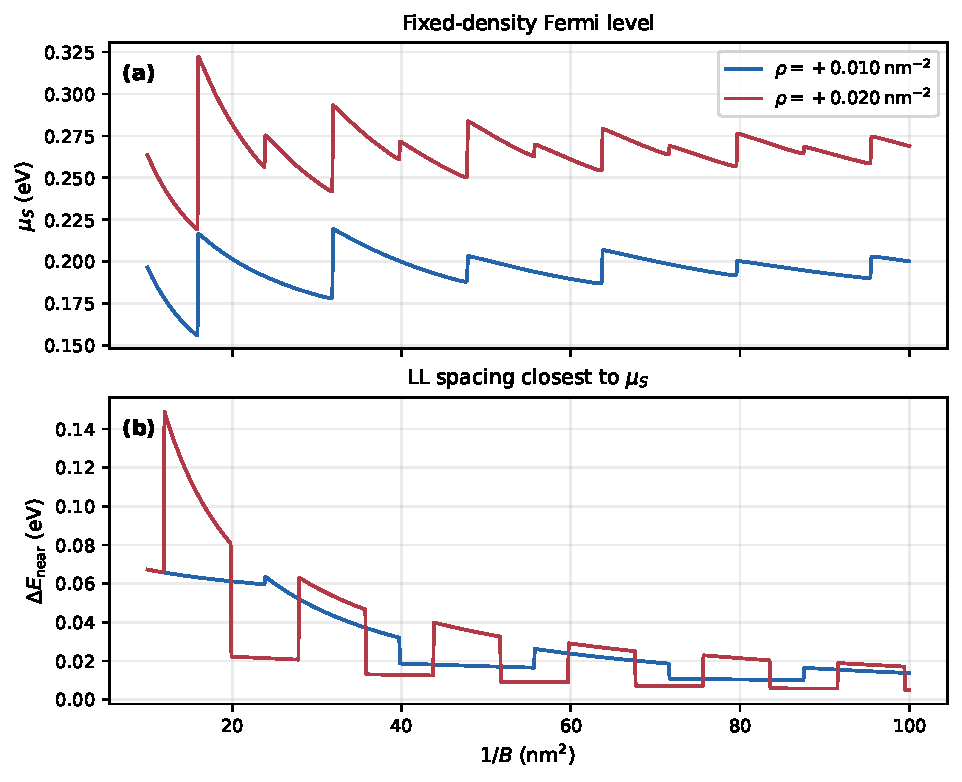
\includegraphics[width=0.86\linewidth]{../figures/spin_counting_diagnostics/electron_mu_and_near_fermi_splitting_comparison.pdf}
    \caption{Comparison of the two electron-density cases used in Figs.~\ref{fig:thermo-wide-osc} and \ref{fig:magnetization-fft}. Panel (a) shows the fixed-density chemical potential \(\mu_{\mathcal S}(1/B)\) for \(\rho=+0.010\) and \(+0.020\,\mathrm{nm}^{-2}\) at \(k_B T=2.0\times10^{-4}\,\mathrm{eV}\). Panel (b) shows the nearest-chemical-potential LL spacing \(\Delta E_{\mathrm{near}}=E_{\mathrm{above}}-E_{\mathrm{below}}\), where \(E_{\mathrm{below}}<\mu_{\mathcal S}<E_{\mathrm{above}}\) are the two LLs closest to the fixed-density chemical potential. }
    \label{fig:electron-mu-splitting-comparison}
\end{figure}

\subsection{Local window selection}

To resolve the thermal damping factor, we need to extract the oscillation amplitude as a function of temperature for the local $1/B$ windows of strong oscillation period, rather than a single global FFT. 
The windows are chosen from the lowest-temperature $\widetilde M_{\mathrm{no0LL}}$ trace and then held fixed for all temperatures.
Operationally, we first identify zero crossings of the oscillatory trace and use same-slope zero crossings to define full local cycles. Fig.~\ref{fig:local-window-selection} shows the resulting $W_0$, $W_1$, and $W_2$ windows.
For $\rho=+0.020\,\mathrm{nm}^{-2}$,
Fig.~\ref{fig:magnetization-fft}(b) shows dominant magnetization weight near
the lower frequency $F=\pi\rho$. The windows in
Fig.~\ref{fig:local-window-selection}(a) therefore follow the corresponding
dominant zero-to-zero cycles; the smaller shoulders are not treated as
independent windows.


\begin{figure}[htbp]
    \centering
    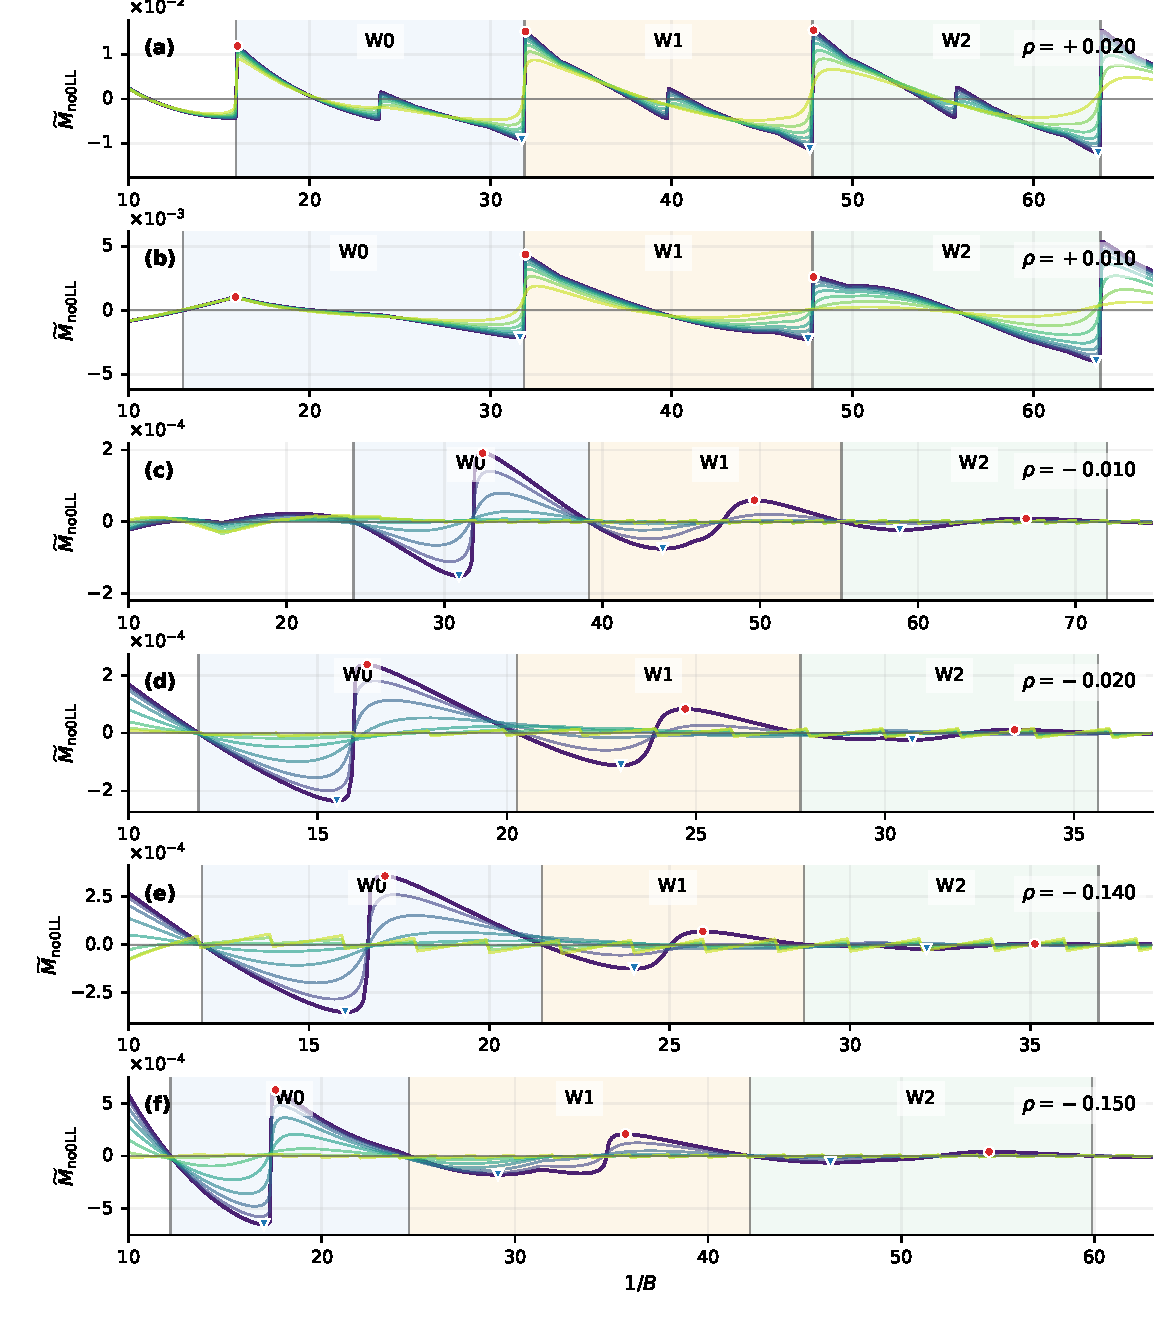
\includegraphics[width=\linewidth]{../figures/appendix_numerics_fresh/appD3_lambda1_zero_aligned_windows.pdf}
    \caption{Local window selection for the zero-mode-excluded oscillatory magnetization at $\Lambda=1.0\,\mathrm{nm}^{-1}$. Each row shows $\widetilde M_{\mathrm{no0LL}}(1/B)$ for one density, with the same temperature sequence as Fig.~\ref{fig:thermo-wide-osc}. Shaded regions mark the three windows $W_0$, $W_1$, and $W_2$ used for local amplitude extraction; red circles and blue triangles mark the maximum and minimum of the lowest-temperature trace in each window.}
    \label{fig:local-window-selection}
\end{figure}

Table~\ref{tab:local-window-periods} compares the selected windows with the expected period $1/F$.
For $\rho=+0.020\,\mathrm{nm}^{-2}$ we track only the main spin-degenerate-like LL oscillation in Fig.~\ref{fig:local-window-selection}(a), so the table uses \(F=\pi\rho\).
For the other densities, the windows follow the spin-resolved active-density counting frequency, \(F=2\pi\rho_{\mathcal S}\), with \(\rho_{\mathcal S}=|\rho|\) for the electron and shallow-hole rows and \(\rho_{\mathcal S}=\rho_{\mathrm{low},e}\) for the deep-hole rows.
Because the numerical waveform is not a perfect sinusoid, individual zero-aligned windows can be slightly uneven; the final column checks the total span of the three selected windows against $3/F$ and gives a value close to unity for all densities, suggesting the correct assignment of the local windows to the expected oscillation period.

\begin{table}[htbp]
    \caption{Local window ranges in $x=1/B$ for Fig.~\ref{fig:local-window-selection}. For $\rho=+0.020\,\mathrm{nm}^{-2}$, the period is evaluated using the main spin-degenerate-like frequency $F=\pi\rho$; for the other rows, it is evaluated using the spin-resolved active-density frequency $F=2\pi\rho_{\mathcal S}$. The last column compares the combined three-window span with three ideal periods.}
    \label{tab:local-window-periods}
    \centering
    \begin{ruledtabular}
    \begin{tabular}{c c c c c c}
        $\rho$ & $W_0$ & $W_1$ & $W_2$ & $1/F$ & $\sum_i\Delta x_i/(3/F)$ \\
        \hline
        $+0.020$ & $[15.933,31.862]$ & $[31.862,47.784]$ & $[47.784,63.703]$ & $15.915$ & $1.000$ \\
        $+0.010$ & $[12.992,31.857]$ & $[31.857,47.787]$ & $[47.787,63.700]$ & $15.915$ & $1.062$ \\
        $-0.010$ & $[24.238,39.150]$ & $[39.150,55.161]$ & $[55.161,71.995]$ & $15.915$ & $1.000$ \\
        $-0.020$ & $[11.842,20.265]$ & $[20.265,27.766]$ & $[27.766,35.639]$ & $7.958$ & $0.997$ \\
        $-0.140$ & $[12.036,21.459]$ & $[21.459,28.727]$ & $[28.727,36.892]$ & $8.309$ & $0.997$ \\
        $-0.150$ & $[12.157,24.523]$ & $[24.523,42.184]$ & $[42.184,59.880]$ & $17.385$ & $0.915$ \\
    \end{tabular}
    \end{ruledtabular}
\end{table}

\subsection{Thermal damping of Normalized oscillation amplitude}

Figure~\ref{fig:window-p1-damping} is obtained directly from the windowed oscillatory magnetization in Fig.~\ref{fig:local-window-selection}.
For each density, temperature, and local window \(w=W_0,W_1,W_2\), we first restrict the background-subtracted trace \(\widetilde M_{\mathrm{no0LL}}(x,T)\), with \(x=1/B\), to the window interval \([x_{w,0},x_{w,1}]\) listed in Table~\ref{tab:local-window-periods}.
The frequency \(F_w\) is the same active-density counting frequency used to choose the window: for \(\rho=+0.020\,\mathrm{nm}^{-2}\) it is the main spin-degenerate-like frequency \(F_w=\pi\rho\), while for the other rows it is \(F_w=2\pi\rho_{\mathcal S}\).
Within this fixed window, the fundamental \(p=1\) harmonic is extracted by the linear projection
\begin{equation}
    \widetilde M_{\mathrm{no0LL}}(x,T)
    =
    C_{1,w}(T)\cos(2\pi F_w x)+S_{1,w}(T)\sin(2\pi F_w x)+C_{0,w}(T).
    \label{eq:window-p1-fit-app}
\end{equation}
The numerical amplitude plotted by the solid markers is
\begin{equation}
    \mathcal R_{1,w}^{\mathrm{num}}(T)
    =
    \frac{A_{1,w}(T)}{A_{1,w}(T_{\min})},
    \qquad
    A_{1,w}(T)=\sqrt{C_{1,w}^{2}(T)+S_{1,w}^{2}(T)}.
    \label{eq:window-p1-normalized-app}
\end{equation}
For \(\rho=-0.020\) and \(-0.140\,\mathrm{nm}^{-2}\), the \(W_2\) amplitudes are too small for a reliable normalized damping curve, so those two \(W_2\) series are not shown.

The dashed curves in Fig.~\ref{fig:window-p1-damping} are then obtained by fitting the normalized amplitudes in each window to the standard LK thermal form
\begin{equation}
    \mathcal R_{1,w}^{\mathrm{LK}}(T;m_w)
    =
    \frac{R_T(T,m_w,\bar B_w)}
    {R_T(T_{\min},m_w,\bar B_w)},
    \qquad
    R_T=\frac{X}{\sinh X},
    \qquad
    X=\frac{2\pi^2 k_B T\,m_w}{\bar B_w}.
    \label{eq:window-lk-fit-app}
\end{equation}
Here \(\bar B_w=1/[(x_{w,0}+x_{w,1})/2]\) is the representative field of the window, and \(m_w\) is the effective mass.
Here we treat \(m_w\) as a single free fitting parameter, rather than using the branch-resolved analytical mass from Sec.~\ref{app:LL-spacing-formulas}.
The fitted \(m_w\) is summarized and compared with the branch-resolved expectation in Fig.~\ref{fig:window-meff-summary}.

The branch-resolved LK expressions explain the scales and behaviors of these fitted masses.
Using the local spacings from Sec.~\ref{app:LL-spacing-formulas}, the LK thermal factor for a single branch is
\begin{equation}
    R_T^{\alpha,\eta}(p,T)
    =
    \frac{X_p^{\alpha,\eta}}{\sinh X_p^{\alpha,\eta}},
    \qquad
    X_p^{\alpha,\eta}
    =
    \frac{2\pi^2 p\kB T}{v_\mu^{\alpha,\eta}}.
    \label{eq:RT-branch-app}
\end{equation}
Writing $\dmu=\mu-E_0$ and substituting the upper-branch spacings from Eq.~\eqref{eq:dEdn-upper-app} together with the lower-branch spacings from Eqs.~\eqref{eq:dEdn-LLminus-app} and \eqref{eq:dEdn-LLTR-app}, the corresponding branch-resolved arguments are
\begin{align}
    X_p^{\uparrow,+}
    &=
    \frac{\pi^2 p\kB T}{aB}
    \frac{\dmu^2-c^2B}{\dmu^2},
    \qquad
    X_p^{\downarrow,+}
    =
    \frac{\pi^2 p\kB T}{aB}
    \frac{\dmu^2+c^2B}{\dmu^2},
    \label{eq:Xp-normal-branch-app}
    \\
    X_p^{\uparrow,-}
    &=
    \frac{\pi^2 p\kB T}{aB}
    \frac{c^2B-\dmu^2}{\dmu^2},
    \qquad
    X_p^{\downarrow,-}
    =
    \frac{\pi^2 p\kB T}{aB}
    \frac{\dmu^2+c^2B}{\dmu^2}.
    \label{eq:Xp-anomalous-branch-app}
\end{align}
The upper-branch expressions apply in the normal dispersive regime, while the lower-branch expressions apply in the anomalous regime within their corresponding crossing windows.
For $\dmu^2\gg c^2B$, both normal expressions reduce to the parabolic result $X_p\simeq\pi^2p\kB T/(aB)$.
For anomalous LLs in the lower-branch crossing windows, \(0<\dmu<c\sqrt{B}\) for \(\ELLminus\) and \(-c\sqrt{B}<\dmu<0\) for \(\ELLTRminus\), the small local spacing makes \(X_p\) much larger at the same \(B\) and \(T\).
In the anomalous regime, where one lower branch dominates a given crossing window, the normalized damping is therefore well represented by the single-branch ratio
\begin{equation}
    \mathcal{R}^{\alpha,-}_{p=1}(\rho,B,T)
    =
    \frac{R_T^{\alpha,-}(p=1,\rho,B,T)}
    {R_T^{\alpha,-}(p=1,\rho,B,T_{\min})}.
    \label{eq:RT-normalized-app-anomalousLL}
\end{equation}
For normal electron doping, the two upper branches lie in the same energy range and are counted together at fixed density.
The fixed-density chemical potential is obtained from
\begin{equation}
    \rho
    =
    \frac{B}{2\pi}
    \sum_{\alpha=\uparrow,\downarrow}
    \sum_{n}
    f\!\left(E^\alpha_{+}(n,B)-\mu_{\rho}\right),
    \label{eq:normal-fixed-density-count-app}
\end{equation}
and the two upper-branch contributions combine at the harmonic-amplitude level as
\begin{equation}
    A^{+}_{p}(\rho,B,T)
    \propto
    \sum_{\alpha=\uparrow,\downarrow}
    v_\mu^{\alpha,+}
    R_T^{\alpha,+}(p,T)
    \cos\!\left(2\pi p n^*_{\alpha,+}\right),
    \qquad
    \mathcal{R}_p^{+}(\rho,B,T)
    =
    \frac{\left|A^{+}_{p}(\rho,B,T)\right|}
    {\left|A^{+}_{p}(\rho,B,T_{\min})\right|}.
    \label{eq:normal-combined-RT-app}
\end{equation}
Here \(E^\alpha_{+}(n^*_{\alpha,+},B)=\mu_{\rho}\).
Equation~\eqref{eq:normal-combined-RT-app} gives the coherent physical harmonic expected from the analytical LK expression, whereas Fig.~\ref{fig:window-p1-damping} uses the simpler fitted form in Eq.~\eqref{eq:window-lk-fit-app} as a local numerical diagnostic of the thermal scale.
The normal electron densities show weak thermal damping over this temperature range, whereas the anomalous-hole densities lose their \(p=1\) amplitude much more rapidly.

\begin{figure}[htbp]
    \centering
    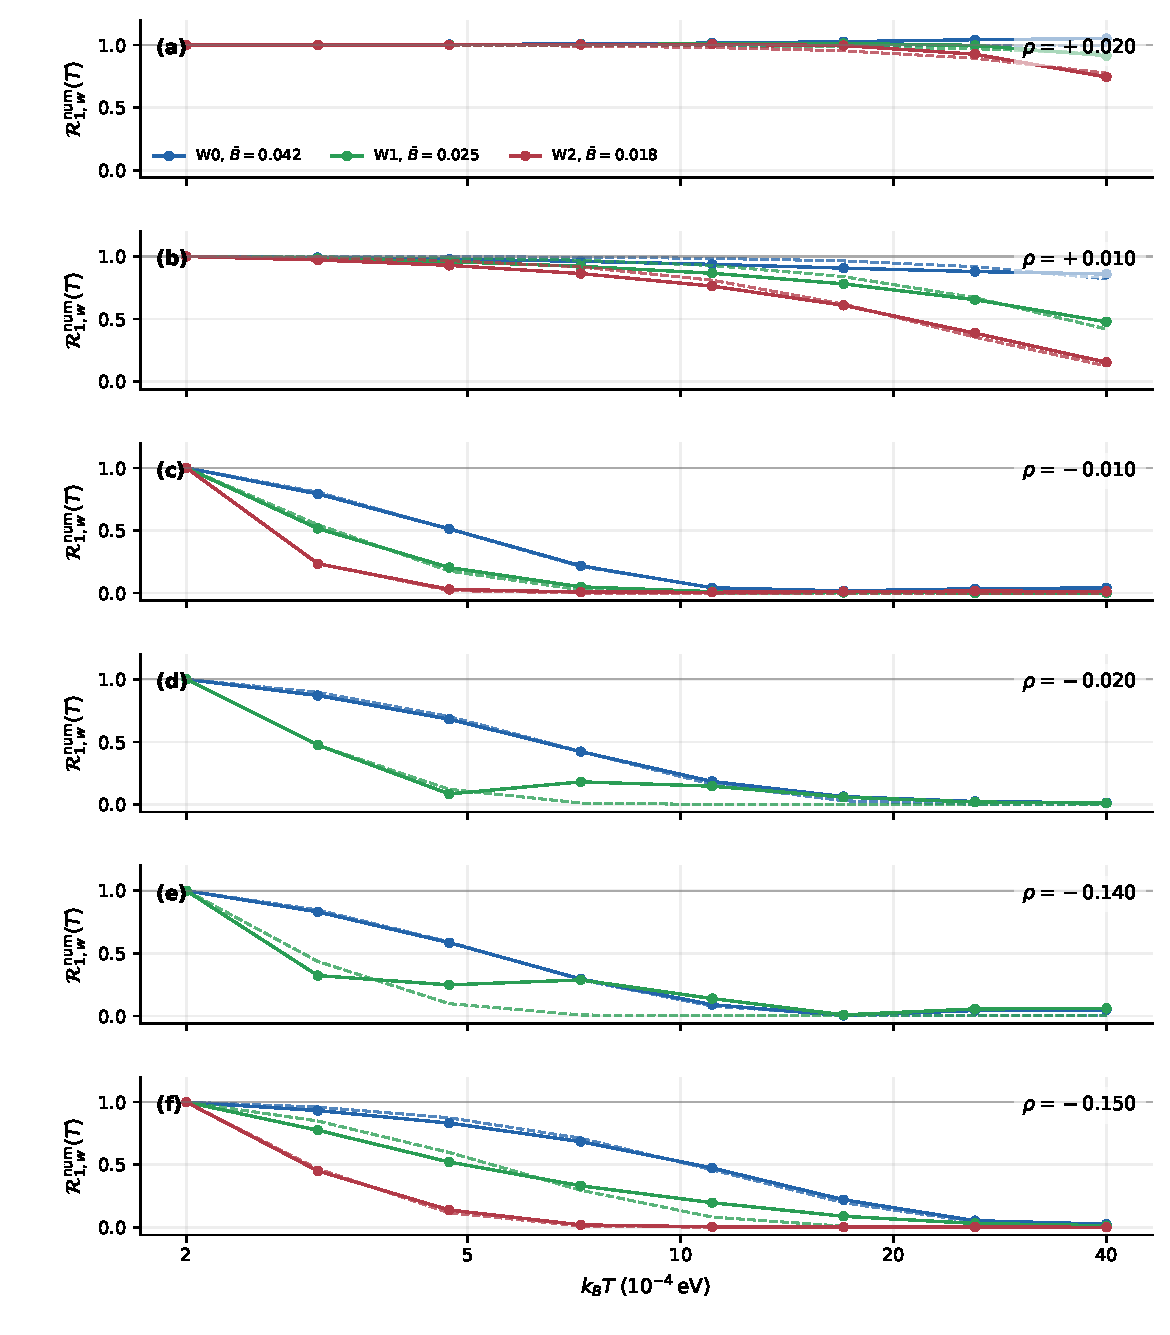
\includegraphics[width=\linewidth]{../figures/appendix_numerics_fresh/appD4_lambda1_window_p1_damping_Rnum.pdf}
    \caption{Windowed \(p=1\) thermal damping extracted from the Fig.~\ref{fig:local-window-selection} windows. Solid markers show the normalized numerical amplitude \(\mathcal R^{\mathrm{num}}_{1,w}(T)\) defined in Eq.~\eqref{eq:window-p1-normalized-app}; dashed curves are one-parameter standard-LK fits for the same window. Three colors blue, green and red label \(W_0\), \(W_1\), and \(W_2\), respectively, and the legend gives the representative field \(\bar B_w\) for the first row. The \(W_2\) series for \(\rho=-0.020\) and \(-0.140\,\mathrm{nm}^{-2}\) are omitted because their amplitudes are too small for reliable damping extraction.}
    \label{fig:window-p1-damping}
\end{figure}

\subsection{Effective masses from the windowed damping}

The fitted standard-LK masses from the dashed curves in Fig.~\ref{fig:window-p1-damping} are summarized in Table~\ref{tab:window-meff-fit-summary} and Fig.~\ref{fig:window-meff-summary}. The standard-LK fits in Fig.~\ref{fig:window-p1-damping} use only the local \(p=1\) harmonic and should therefore be read as qualitative thermal-scale diagnostics rather than precision measurements of a unique band mass. Because the numerical waveform is not a pure sinusoid, as clearly shown in Fig.~\ref{fig:local-window-selection}, the higher harmonics \(p>1\) is also not negligible, but we only focus on $p=1$ harmonic in the current analysis of effective mass below. 

Each marker in Fig.~\ref{fig:window-meff-summary} corresponds to the extracted effective mass for one window and is placed at the representative field \(\bar B_w\).
The curves show the branch-resolved analytical expectation \(m^*_{\mathrm{eff}}(B)=B/v_\mu\) from Sec.~\ref{app:lk-branch}; for normal electron densities we show both nearby upper branches, while for anomalous-hole densities we show the active lower branch selected by the fixed-density counting.
Figure~\ref{fig:window-meff-summary}(a) shows the effective mass for the normal LLs in electron carrier regime.
Except for the first \(\rho=+0.020\,\mathrm{nm}^{-2}\) window, the fitted masses remain of order unity and lie around the parabolic scale \(1/(2a)\), with visible window-to-window variation because the two upper branches, \(\ELLplus\) and \(\ELLTRplus\), contribute in the same energy range and are not exactly degenerate. For \(\rho=+0.020\,\mathrm{nm}^{-2}\), we note that the projected \(p=1\) amplitude is nearly temperature independent and even increases slightly with temperature, as shown in Fig.~\ref{fig:window-p1-damping}a, so the one-parameter LK fit returns a mass close to zero. This suggests the higher harmonics ($p>1$) also plays important role in the temperature dependence of the oscillation amplitude in this window, beyond the current $p=1$ harmonics fitting. Fig.~\ref{fig:window-meff-summary}(b) shows the effective mass of anomalous LLs in hole carrier regime.
The fitted masses are much larger and more field dependent, qualitatively following the trend of the active lower-branch analytical curves. This is the mass-scale version of the rapid thermal damping in Fig.~\ref{fig:window-p1-damping}: the anomalous LL spacing is much smaller, so the LK argument \(X\propto m^*_{\mathrm{eff}}T/B\) is much larger at comparable \(B\) and \(T\). However, the fitted masses are quantitatively deviated from the analytical branch-resolved curves in Fig.~\ref{fig:window-meff-summary}(b), suggesting the limitation of the effective mass description of the thermal damping in the anomalous LL regime. 


\begin{table}[htbp]
    \caption{Fitted standard-LK masses \(m_w\) extracted from the dashed curves in Fig.~\ref{fig:window-p1-damping} and plotted in Fig.~\ref{fig:window-meff-summary}. The entries correspond to the local windows \(W_0,W_1,W_2\) defined in Fig.~\ref{fig:local-window-selection}. }
    \label{tab:window-meff-fit-summary}
    \begin{ruledtabular}
    \begin{tabular}{ccccc}
        \(\rho\,(\mathrm{nm}^{-2})\) & regime & \(m_{W_0}\) & \(m_{W_1}\) & \(m_{W_2}\) \\
        \hline
        \(+0.020\) & normal LL & \(1.04\times10^{-4}\) & \(0.206\) & \(0.288\) \\
        \(+0.010\) & normal LL & \(0.626\) & \(0.788\) & \(0.958\) \\
        \(-0.010\) & anomalous LL & \(8.27\) & \(10.2\) & \(13.9\) \\
        \(-0.020\) & anomalous LL & \(11.3\) & \(23.0\) & -- \\
        \(-0.140\) & anomalous LL & \(13.6\) & \(23.7\) & -- \\
        \(-0.150\) & anomalous LL & \(5.92\) & \(6.73\) & \(11.0\) \\
    \end{tabular}
    \end{ruledtabular}
\end{table}

\begin{figure}[htbp]
    \centering
    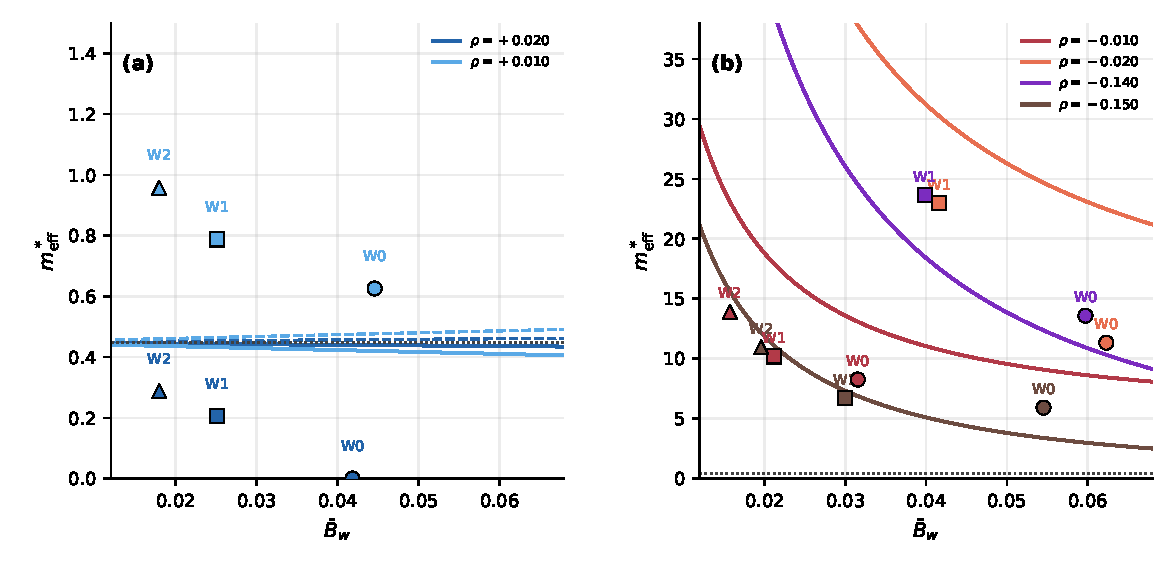
\includegraphics[width=\linewidth]{../figures/appendix_numerics_fresh/appD5_lambda1_effective_mass_summary.pdf}
    \caption{Effective masses extracted from the Fig.~\ref{fig:window-p1-damping} standard-LK fits. Panel (a) shows the normal electron windows for \(\rho=+0.020\) and \(+0.010\,\mathrm{nm}^{-2}\), with analytical curves for the nearby \(\ELLplus\) and \(\ELLTRplus\) upper branches; the near-zero \(W_0\) point for \(\rho=+0.020\,\mathrm{nm}^{-2}\) reflects the nearly non-damping projected \(p=1\) amplitude in that window. Panel (b) shows the anomalous-hole windows for \(\rho=-0.010,-0.020,-0.140\), and \(-0.150\,\mathrm{nm}^{-2}\), with analytical curves for the active lower branch selected by the fixed-density counting; the \(W_2\) points for \(\rho=-0.020\) and \(-0.140\,\mathrm{nm}^{-2}\) are omitted because their amplitudes are too small for reliable extraction. Markers are fitted masses for the local windows, labelled by \(W_0,W_1,W_2\) when shown. The dotted horizontal line marks the parabolic value \(1/(2a)\).}
    \label{fig:window-meff-summary}
\end{figure}





% ================================================================

\appendixmaybeenddocument
